%%% ArXiv template from https://www.overleaf.com/latex/templates/an-arxiv-template/gbzmznbxvwpr

\documentclass{article}

\usepackage{graphicx}
\usepackage{indentfirst,csquotes}
\usepackage{amssymb,amsthm,amsmath}
\usepackage{xcolor,paralist,hyperref,fancyhdr,etoolbox,cleveref}
\usepackage[square,sort,comma,numbers]{natbib}
\usepackage{algorithm}
\usepackage{algpseudocode}
\usepackage{subcaption}
\usepackage{tikz-cd}
\usetikzlibrary{positioning, fit, backgrounds, arrows.meta}
\usepackage{enumitem}
\allowdisplaybreaks
\numberwithin{equation}{section}
\hypersetup{colorlinks=true, linkcolor=black, filecolor=black, urlcolor=black}

\baselineskip=16pt
\topmargin= .5cm
\textheight= 20cm
\textwidth= 32cc
\baselineskip=16pt

\evensidemargin= .9cm
\oddsidemargin= .9cm



\theoremstyle{plain}
\newtheorem{theorem}{Theorem}[section]
\newtheorem{definition}{Definition}[section]
\newtheorem{example}[theorem]{Example}
\newtheorem{lemma}{Lemma}[section]
\newtheorem{proposition}[theorem]{Proposition}
\newtheorem{corollary}[theorem]{Corollary}
\newtheorem{conjecture}[theorem]{Conjecture}
\newtheorem{assumption}{Assumption}
\newtheorem{remark}{Remark}



\def\proof{\noindent {\it Proof. $\, $}}
\def\endproof{\hfill $\Box$ \vskip 5 pt }


%%% PERSONAL ADD-ONS



\include{macros}

\newcommand{\inner}[2]{\left\langle {#1} , {#2} \right\rangle} % inner product
\newcommand{\proj}[2]{P_{#1} \left[ {#2} \right]} % Projection 
% For foot notes in author name
\newcommand{\footremember}[2]{%
	\footnote{#2}
	\newcounter{#1}
	\setcounter{#1}{\value{footnote}}%
}
\newcommand{\footrecall}[1]{%
	\footnotemark[\value{#1}]%
} 


% For foot notes / comments
\newif\ifnotes\notestrue

\def\boxnote#1#2{\ifnotes\fbox{\footnote{\ }}\ \footnotetext{ From #1: #2}\fi}
\def\fabian#1{\boxnote{Fabian}{\color{red}#1}}
\def\mfabian#1{{\color{red} #1}}
\def\hfabian#1{}

\def\pierre#1{\boxnote{Pierre}{\color{blue}#1}}
\def\mpierre#1{{\color{blue} #1}}
\def\hpierre#1{}

\def\todo#1{\boxnote{\textbf{TODO}}{#1}}
\def\mtodo#1{{#1}}
\def\htodo#1{}

\title{An augmented Lagrangian algorithm for constrained nonlinear least-squares} %%%%%%%%%%%%

\author{Pierre Borie\footremember{udem}{University of Montreal, Department of Computer Science and Operations Research, Montreal, QC, Canada}, Fabian Bastin\footrecall{udem}, Stéphane Dellacherie\footremember{hq}{Hydro-Québec, Montreal, QC, Canada}\footremember{uqam}{Université du Québec à Montréal, Montreal, QC, Canada}}


\begin{document}
	


\date{\today}

\maketitle
		
\begin{abstract}
\noindent We present an algorithm for solving nonlinear least-squares problems subject to a mix of nonlinear and linear constraints. The nonlinear constraints are handled by reformulating the objective as the augmented Lagrangian function while linear constraints are handled directly. Each iteration consists in approximately solving a linearly constrained problem by means of a gradient projection technique. Our approach also involves a structured approximation of the augmented Lagrangian Hessian. We show global convergence of the method and provide numerical experiments.

\vspace{1em}\noindent\textbf{Keywords:} constrained nonlinear least-squares, augmented Lagrangian method, Julia, structured quasi-Newton update. 
\end{abstract} %%%%%%%%% 

\section{Introduction}

We consider the constrained nonlinear least-squares (NLS) problem
\begin{equation}
	\label{pb:cnls}
	\begin{aligned}
		\min_{x\in \RR^n} \quad & \dfrac{1}{2} \|r(x)\|^2 \\
		\text{s.t.} \quad & c(x) = 0 \\
		& x \in \Omega
	\end{aligned}
\end{equation}
where $\|\cdot\|$ denotes the $\ell_2$ norm. The residuals $r\colon \RR^n \to \RR^{n_r}$ and constraints $c\colon \RR^n \to \RR^{n_c}$ functions are assumed to be twice continuously differentiable with respective Jacobian $J$ and $C$. We may also write the least-squares objective as a general function $f$ with gradient 
\[\nabla f(x) = J(x)^\top r(x).\] 
The set $\Omega$ consists of linear constraints and is defined as
\begin{equation}\label{eq:linear_constraints}
	\Omega = \left\{ x \in \RR^n \ | \ Ax=b,\ l \le x \le u\right\},
\end{equation}
with $A\in\RR^{m\times n}$, $m < n$, $b\in \RR^m$, and $l,u \in \RR^n$. Without loss of generality, some components of the latter two vectors can be set to $\pm \infty$ for unbounded parameters. For convenience, we also assume that the linear equalities do not involve single-variable constraints. Formulation~\eqref{pb:cnls} is also suitable for problems with nonlinear inequality constraints of the form $g(x) \ge 0$. The latter are transformed into equality constraints by adding non-negative slack variables, which gives the new constraints
\begin{equation*}
	g(x) - \nu = 0,\quad \nu \ge 0.
\end{equation*}
The lower and upper bounds associated to these slack variables are thus $0$ and $\infty$ respectively. Linear inequality constraints can be converted into equalities similarly.

The Lagrangian for problem~\eqref{pb:cnls}, with respect to the nonlinear constraints, is defined by 
\begin{equation*}
	\calL(x,\lambda) = f(x) + \inner{\lambda}{c(x)},
\end{equation*}
where $\lambda \in \RR^{n_c}$ is the vector of Lagrange multipliers and $\inner{\cdot}{\cdot}$ is the standard inner product.

An algorithm for solving problem~\eqref{pb:cnls} aims to find a first-order critical point $(x_*,\lambda_*)$ that satisfies the necessary condition
\begin{equation*}
	\begin{aligned}
		&x_* \in \Omega\ \text{and}\ c(x_*)=0 \\
		&\proj{\Omega}{x_*-\nabla_x \calL(x_*,\lambda_*)}=x_*,
	\end{aligned}
\end{equation*}
where $\proj{\Omega}{\cdot}$ is the projector operator onto $\Omega$, defined, for any vector $x$, as
\begin{equation*}
	\proj{\Omega}{x}= \argmin_{v\in \Omega} \ \|v-x\|^2. 
\end{equation*}

The NLS structure arises naturally in data fitting, parameter estimation, and scientific computing, and its efficient resolution has attracted a sustained research effort~\cite{dennisschnabel:1996,nocedalwright:2006,bjork:2024}. 
A distinctive feature of NLS problems is that the Hessian of the objective decomposes into a first-order part $J(x)^\top J(x)$, where $J(x)$ is the Jacobian of $r$, and second-order part involving the individual Hessians of the residuals weighted by their values. Exploiting this decomposition is the central challenge in designing
efficient algorithms.
The Gauss--Newton (GN) method~\cite[][Chapter 9]{dennisschnabel:1996} retains only the first-order term, which is effective when residuals are small at the solution but can lead to poor convergence otherwise.
The Levenberg--Marquardt (LM) method, initiated in~\cite{levenberg:1944,	marquardt:1963} and further studied, for instance, in~\cite{bellavia-etal:2018,	bergou-etal:2021}, regularizes the GN matrix by a scalar multiple of the identity, providing robustness at the cost of potentially slower convergence on large-residual problems.
A richer class of approaches, known as structured quasi-Newton (SQN) methods, approximates the second-order part through secant equations tailored to the least-squares structure. The NL2SOL package~\cite{dennisetal:1981,dennis-etal:1989} is a popular implementation of this idea, complementing the GN term with a structured quasi-Newton correction updated via a dedicated secant equation. This algorithm also switches between the GN model or the full Hessian depending on the quality of the step. Other hybrid strategies with switching criterion based on the residual magnitude have also been explored in~\cite{albaalifletcher:1985, fletcherxu:1987, zhouchen:2010}. Further SQN formulations, including factorized updates and sizing strategies, have been proposed in~\cite{biggs:1977, betts:1976, huschens1994, yabetakahashi:1991, zhang-etal:2000}. A comprehensive numerical comparison of these techniques can be found in~\cite{lucksan-etal:2019}.

Extending structured NLS methods to the constrained setting has received comparatively less attention, though it remains an active area of research. Such formulations arise, for example, in data-fitting problems where the constraints enforce the physical consistency of an underlying model~\cite{grenieretal:2006, delbos-etal2006, pu-etal:2015}. The convex case, especially the bound constrained case, is studied in~\cite{bellavia-etal:2004, bellavia-etal:2011, porcelli:2013, goncalvesmenezes:2020}.
For more general nonlinear constraints, most methods operate within a sequential quadratic programming (SQP) framework. In that paradigm, each iteration solves a quadratic subproblem obtained by linearizing the constraints and approximating the Hessian of the Lagrangian. \cite{li-etal:2002} propose an SQP method whose Hessian approximation
is based on a secant equation derived from~\cite{biggs:1977}; \cite{tjoabiegler:1991} use a BFGS update of the projected Hessian of a merit function; and~\cite{amiribartels:1989} update the structured  approximation projected Hessian in the null space of the active constraints.
For problems with equality constraints only, more recent work includes regularized approaches: \cite{bergou-etal:2021} combine a Levenberg--Marquardt approximation of the Lagrangian Hessian with a trust-region method, and~\cite{orbansiquiera:2020} derive a regularized KKT system by adding primal and dual regularization terms.
Structured approximations of the Hessian within general constrained	formulations have also been studied from a theoretical perspective in~\cite{tapia:1988}.

When the constraints can be split into two categories, as in formulation~\eqref{pb:cnls}, an alternative to SQP methods is the augmented Lagrangian (AL) framework, also known as the method of multipliers, independently introduced by~\cite{hestenes:1969} and~\cite{powell:1969}, with further theoretical foundations provided by~\cite{rockafellar:1973}.
Rather than solving a sequence of quadratic subproblems, AL methods incorporate the nonlinear constraints into the objective as a penalty term and solve a sequence of subproblems in which only the easier constraints remain.
For problem~\eqref{pb:cnls}, this amounts to approximately minimizing, at each outer iteration, the AL function over the polyhedral set $\Omega$, thereby reducing the problem to a linearly constrained one. This strategy is particularly attractive as the linear part can be handled directly and efficiently by gradient projection techniques, without sacrificing the ability to enforce nonlinear constraints.
The theoretical underpinnings of this approach, including global convergence results, are developed in~\cite{conn-etal:1988a,conn-etal:1991, conn-etal:1993, conn-etal:1996b} and summarized	in~\cite[][Chapter~14]{conn-etal:2000}.
A major implementation of this philosophy is the LANCELOT solver~\cite{conn-etal:1992}, which handles bound-constrained
subproblems using a gradient projection technique~\cite{conn-etal:1988b}.
More recent AL implementations have broadened this framework in several	directions: \cite{andreani-etal:2008} establish convergence under
weaker constraint qualifications; \cite{gillrobinson:2012} propose a primal-dual AL method that behaves like a stabilized SQP method in the local regime; \cite{arreckx-etal:2016} implement a matrix-free AL approach and \cite{curtis-etal:2015} develop an adaptive AL algorithm with inexact subproblem solves.
For the inner minimization that arises at each outer AL iteration, gradient projection methods~\cite{moretoraldo:1991, linmore:1999a} are particularly effective for bound-constrained problems as they allow for rapid changes in the active set throughout the iterations. The linear equality case can be handled efficiently, as the projections can be computed by solving a system of normal equations~\cite{gould-etal:2001}.
When both bounds and linear equalities are present, as in our setting, direct projection onto $\Omega$ is not available in closed form. Nevertheless, we will see in the next section that the norm of the reduced gradient provides a practical criticality measure, as used in solvers such as MINOS~\cite{murtaghsaunders:1978} and LSNNO~\cite{tointtuyttens:1992}.

The present work combines two well-established lines of research: the augmented Lagrangian framework of Conn, Gould, and Toint~\cite{conn-etal:1988a, conn-etal:1991, conn-etal:1993, conn-etal:1996b, conn-etal:2000}, with its mature convergence theory and gradient projection inner minimization, and the quasi-Newton approximations that exploit the sum-of-squares structure of both the objective and the penalty term, following the secant equation philosophy of~\cite{biggs:1977,dennisetal:1981} adapted to the AL setting in the spirit of~\cite{li-etal:2002}. Bringing these together yields a solver specifically designed for NLS problems while handling constraints of general form, including nonlinear equalities and inequalities alongside linear equalities and bounds. Our algorithm is implemented in the Julia programming language~\cite{bezanson-etal:2017} and is open-source.

We end this section by introducing some notations. Jacobian matrices of $r$ and $c$ evaluated at $x$ are respectively noted $J(x)$ and $C(x)$. Components of a vector $x\in\RR^n$ are noted $x_i$ for $i=1,\ldots,n$. Vectors $e_i$ denote the columns of the $n \times n$ identity matrix. When describing iterative processes to solve problem~\eqref{pb:cnls}, we index vectors and matrices by the iteration number. For instance, at iteration $k$, $(x_k,\lambda_k)$ is the current primal-dual iterate. For functions evaluated at $x_k$, we use the shorthand notation $r_k = r(x_k)$, $c_k =c(x_k)$, $J_k=J(x_k)$ etc. To not interfere with previous notation for components, we add parentheses to make the distinction clear. For instance, $(x_k)_i$ denotes the $i$-th component of vector $x_k$. For any sequence $(u_k)_k$, the limit of a converging subsequence indexed by $\calK \subset \NN$ will be written $\lim\limits_{k \in \calK} u_k$. The orthogonal complement of a subspace $V \subset \RR^n$, i.e. the set $\{ w\ | \ \inner{w}{v}=0\ \text{for all}\ v \in V\}$, will be written $V^\perp$.

The rest of the paper is organized as follows. In Section~\ref{sec:algorithm}, we present our algorithmic framework and discuss implementation details. We study global convergence in Section~\ref{sec:convergence_analysis}. Numerical experiments are shown in Section~\ref{sec:numerical_experiments} and we conclude with perspectives.

\section{Algorithm}\label{sec:algorithm}

\subsection{Augmented Lagrangian framework}\label{subsec:al_framework}

We formally state the first assumptions about problem~\eqref{pb:cnls}.
\begin{assumption}\label{assumption:functions_C2}
	Residuals $r$ and constraints $c$ are twice continuously differentiable on $\RR^n$.
\end{assumption}
\begin{assumption}\label{assumption:full_rank_A}
	The equality constraint matrix $A$ is full row rank.
\end{assumption}
\begin{assumption}\label{assumption:feasible_linear_cons}
	The feasible region for the linear constraints $\Omega$ is non-empty.
\end{assumption}

Our method is based on the Augmented Lagrangian (AL) function defined as
\begin{equation}\label{eq:al}
	\Phi(x,\lambda,\mu) := \dfrac{1}{2}\|r(x)\|^2 + \inner{\lambda}{c(x)} + \dfrac{\mu}{2} \|c(x)\|^2,
\end{equation}
where $\mu > 0$ is a penalty parameter.

We maintain the linear constraints in the formulation of the problem and only penalize the violation of the nonlinear constraints.
One has the following expression for the gradient: 
\begin{equation*}
	\nabla_x \Phi(x,\lambda,\mu) = J(x)^\top r(x) + C(x)^\top\bar{\lambda}(x,\lambda,\mu),
\end{equation*}
where
\begin{equation}\label{eq:1st_order_mult}
	\bar{\lambda}(x,\lambda,\mu):=\lambda + \mu c(x),
\end{equation} 
are the first-order estimates of the Lagrange multipliers. The AL and Lagrangian gradients are related by the identity
\begin{equation}\label{eq:identity_al_lag_grad}
	\nabla_x \Phi(x,\lambda,\mu) = \nabla_x \calL(x,\bar{\lambda}(x,\lambda,\mu)).
\end{equation}
The Hessian is given by
\begin{equation*}
	\nabla^2_{xx} \Phi(x,\lambda,\mu) = J(x)^\top J(x) + \mu C(x)^\top C(x) +  S(x) 
\end{equation*}
with the second-order terms explicitly given by
\begin{equation}\label{eq:al_hessian_2nd_terms}
	S(x) =\sum_{i=1}^{n_r} r_i(x) \nabla^2r_i(x) + \sum_{i=1}^{n_c} \nabla^2 c_i(x) \bar{\lambda}_i(x,\lambda,\mu).
\end{equation}
For fixed $\lambda$ and $\mu$, reformulating problem~\eqref{pb:cnls} with function~\eqref{eq:al} gives the linearly constrained problem
\begin{equation}\label{pb:cnls_al_reformulation} 
	\begin{aligned}
		\min_{x} \quad& \Phi(x,\lambda,\mu)  \\
		\text{s.t.}  \quad & x \in \Omega.
	\end{aligned}	
\end{equation}
Moving the nonlinear constraints into the objective simplifies the problem because only linear constraints are left, which enables one to use iterative methods for linearly constrained optimization while still improving feasibility of the nonlinear constraints. Since $\Omega$ is a convex set, a first-order critical point of~\eqref{pb:cnls_al_reformulation} can also be characterized by the condition
\begin{equation*}
	\proj{\Omega}{x^*-\nabla_x \Phi(x^*,\lambda,\mu)} = x^*.
\end{equation*}
In our methods, and as in standard AL methods, each iterate $x_k$ is an approximate solution of a subproblem of the form~\eqref{pb:cnls_al_reformulation} satisfying
\begin{equation}\label{eq:algo_traulls_criticality_test}
	\|\proj{\Omega}{x_k-\nabla_x\Phi(x_k, \lambda_k, \mu_k)}-x_k\| \le \omega_k,
\end{equation}
for a fixed vector of multipliers $\lambda_k$, penalty parameter $\mu_k$ and tolerance $\omega_k$.
If the iterate $x_k$ improves the feasibility violation of the nonlinear constraints, a dual ascent step is taken on the Lagrange multipliers by setting
\begin{equation*}
	\lambda_{k+1} = \lambda_k + \mu_k c_k = \bar{\lambda}(x_k,\lambda_k,\mu_k).
\end{equation*}
If on the contrary, feasibility has not been improved, the minimization~\eqref{pb:cnls_al_reformulation} is restarted using an increased penalty parameter $\mu_{k+1} > \mu_k$ to enforce feasibility. The method is outlined in Algorithm~\ref{algo:traulls}. Following our notation for iteration dependent quantities, we respectively write $\nabla_x\Phi(x_k, \lambda_k, \mu_k)$ and $\bar{\lambda}(x_k,\lambda_k,\mu_k)$ in the compact form $\nabla_x \Phi_k$ and $\bar{\lambda}_k$.
\begin{algorithm}
	\caption{Augmented Lagrangian algorithm}\label{algo:traulls}
	\begin{algorithmic}[1]
		\Require Initial starting point $x^s_0 \in \Omega$, Lagrange multipliers estimate $\lambda_0$, penalty parameter $\mu_0$
		\State Penalty parameter increase factor $\tau > 1$, tolerance update constants $\omega,\eta, \kappa_\omega, \kappa_\eta, \beta_\omega, \beta_\eta$
		\State{Set initial tolerances $\omega_0\gets \omega \mu_0^{-\kappa_\omega}$ and $\eta_0\gets \eta \mu_0^{-\kappa_\eta}$}
		\For{k=0,1,2\ldots}
		\State\label{line:inner_iteration} Starting from $x_k^s$, approximately solve $\min_{x\in \Omega} \Phi(x,\lambda_k,\mu_k)$ to find $x_k \in \Omega$ satisfying~\eqref{eq:algo_traulls_criticality_test}.
		\If{$\|c(x_k)\| \le \eta_k$}
		\If{\(\|\proj{\Omega}{x_k-\nabla_x\Phi_k}-x_k\|  \le \omega_*\) and \(\left\Vert c(x_k)\right\Vert \le \eta_*\)}
		\State{\textbf{stop} and} \Return approximate solution $(x_k,\lambda_k)$
		\EndIf
		\State Update the Lagrange multipliers $\lambda_{k+1}\gets \bar{\lambda}_k$ 
		\State Set the next starting point $x_{k+1}^s \gets x_k $
		\State Leave the penalty parameter unchanged \(\mu_{k+1} \gets \mu_k\)
		\State Decrease the tolerances $\omega_{k+1}\gets \omega_k \mu_{k+1}^{-\beta_\omega}$ and $\eta_{k+1}\gets \eta_k \mu_{k+1}^{-\beta_\eta}$
		\Else{}
		\State Let the iterate unchanged \(\left(x_{k+1}^s,\lambda_{k+1}\right) \gets \left(x_k^s,\lambda_k\right)\)
		\State Increase the penalty parameter $\mu_{k+1} \gets \tau\mu_k$
		\State Update tolerances $\omega_{k+1}\gets \omega \mu_{k+1}^{-\kappa_\omega}$ and $\eta_{k+1}\gets \eta \mu_{k+1}^{-\kappa_\eta}$
		\EndIf
		\EndFor
	\end{algorithmic}
\end{algorithm}
One first notices that Algorithm~\ref{algo:traulls} has an outer-inner iteration structure, in the sense that each iteration requires to approximately solve an optimization problem (line~\ref{line:inner_iteration}), which also involves an iterative process. The techniques used for the latter are detailed in Section~\ref{sec:inner_iteration}.

Tolerances in Algorithm~\ref{algo:traulls} are updated in such a way that both sequences $\omega_k$ and $\eta_k$ tend to $0$ when $k \to \infty$. The update scheme that we outline follows the rules described in~\cite[][Chapter 14]{conn-etal:2000}. The parameters values used in our implementation are given in Section~\ref{subsec:implementation_details}.

We describe the convergence in terms of the norm of the projected gradient but this quantity is not easily computable in practice. Indeed, contrary to the case where there is only bounds or linear equality constraints, there is no direct formula for the projection on a polyhedral set of the form $\Omega$. For our implementation, we will use the norm of the reduced gradient, which we define now. 

For $x \in \Omega$, $I^+(x)$, resp. $I^-(x)$ denotes the indices of upper bounds, resp. lower bounds, satisfied as equalities (active) at $x$ and $I(x) := I^+(x) \cup I^-(x)$, i.e.:
\begin{equation*}
	i \in I(x) \implies x_i \in \{l_i,u_i\}.
\end{equation*}
We also introduce the notion of tangent space at a point $x$, written $T(x)$ and defined as the set of directions $d$ such that the same constraints are satisfied with equality at both $x$ and $x+d$. In our case, this corresponds to the linear equality constraints and the active bounds. Formally:
\begin{equation}\label{eq:tangent_space}
	T(x) := \left\{ d \in \RR^n \ | \ Ad = 0,\ d_i=0\ \text{for all}\ i\in I(x)\right\}.
\end{equation}
At a given point \((x,\lambda)\) and parameter $\mu$, the reduced gradient is defined as 
\begin{equation*}
	\proj{T(x)}{\nabla_x \Phi(x,\lambda,\mu)}.
\end{equation*}
Provided that the multipliers associated to the active bounds are of appropriate sign, the quantity $\|\proj{T(x)}{\nabla_x \Phi(x,\lambda,\mu)}\|$ is an appropriate criticality measure used in optimization algorithms for linearly constrained optimization such as MINOS~\cite{murtaghsaunders:1978} and LSNNO~\cite{tointtuyttens:1992}.
Projections on $T(x)$ can be computed in closed form. Indeed, assuming that $I(x) =  \left\{i_1,\ldots, i_p\right\}$ with $p < n-m$ and denoting by $Z \in \RR^{p\times n}$ the matrix whose row $k$ is the row $i_k$ of the $n\times n$ identity matrix, $T(x)$ is nothing but the null space of the block matrix 
\begin{equation}\label{eq:matrix_tangent_space}
	\tilde{A} = \begin{pmatrix}
	A \\Z
\end{pmatrix}.
\end{equation}
Let $\tilde{N}$ be a matrix whose columns form an orthonormal basis of the null space of $\tilde{A}$. By construction and our full rank Assumption~\ref{assumption:full_rank_A}, $\tilde{A}$ is also full rank. Then, the projection of a vector $v$ onto the null space of $\tilde{A}$ is given by $\tilde{P}v$ where
\[\tilde{P} = \tilde{N}\tilde{N}^\top,\]
There is no need to explicitly form the matrix $\tilde{N}$ because we can make use of the equivalent expression of the projection matrix $\tilde{P}$:
\begin{equation}\label{eq:minor_subpb_projector}
	\tilde{P} = I - \tilde{A}^\top\left(\tilde{A}\tilde{A}^\top\right)^{-1}\tilde{A}.
\end{equation}
Using~\eqref{eq:minor_subpb_projector}, one can compute the projection of a vector $v$, i.e. $\tilde{P}v$, by first solving, for an auxiliary variable $y$, the linear system
\begin{equation}\label{eq:proj_normal_eq_auxiliary_syst}
	\left(\tilde{A}\tilde{A}^\top\right)y = \tilde{A}v,
\end{equation}
and retrieve the projection by
\begin{equation*}
	v - \tilde{A}^\top y.
\end{equation*}
This approach, referred as the \textit{normal equations} approach~\cite{gould-etal:2001}, requires to solve the system~\eqref{eq:proj_normal_eq_auxiliary_syst}. This is done by using the Cholesky decomposition of $\tilde{A}\tilde{A}^\top$. The latter is well defined because the matrix $\tilde{A}\tilde{A}^\top$ is symmetric by construction and positive definite by Assumption~\ref{assumption:full_rank_A}. System~\eqref{eq:proj_normal_eq_auxiliary_syst} is reduced to two successive lower triangular systems. The factorization $\tilde{A}\tilde{A}^\top = \tilde{L}\tilde{L}^\top$, with $\tilde{L}$ lower triangular, does not need to be computed from scratch because the structure of $\tilde{A}$ implies a block structured Cholesky factor that involves the Cholesky decomposition of $AA^\top$. The latter is constant throughout the algorithm, so the factor $\tilde{L}$ can be computed in a relatively efficient manner, even though it potentially has to be updated at every new minor iteration. We expect it to be the case when these computations take place in the first outer iterations of Algorithm~\ref{algo:traulls}, but that as we progress toward a first-order critical point, the set of active bounds tends to stabilize and remain the same during the inner iterations. Details on this computation can be found in Appendix~\ref{appendix:chol_aug_matrix}.

This discussion justifies why our implementation uses condition
\begin{equation}\label{eq:criticality_cond_reduced_grad}
	\|\proj{T_k}{\nabla_x\Phi_k}\| \le \omega_k
\end{equation}
in Algorithm~\ref{algo:traulls} instead of~\eqref{eq:algo_traulls_criticality_test}.

\subsection{Inner minimization process}\label{sec:inner_iteration}

In this section, we describe the inner minimization process used to produce the outer iterates of Algorithm~\ref{algo:traulls}.
Since the current multipliers estimates $\lambda$ and the penalty parameter $\mu$ are fixed, the objective function for the inner minimization only depends on $x$ so we use the shorthand notation $\varphi : x\mapsto \Phi(x,\lambda,\mu)$.
Given a point $x_0 \in \Omega$, multipliers estimates $\lambda$, a penalty parameter $\mu$, we aim to find an approximate solution of the problem
\begin{equation}\label{eq:inner_itr_subpb}
	\begin{aligned}
		\min_x \quad & \varphi(x)\\
		\text{s.t.} \quad & x \in \Omega,
	\end{aligned}
\end{equation}
and such that
\begin{equation*}
	\|\proj{T(x)}{\nabla \varphi(x)}\| \le \omega,
\end{equation*}
for a tolerance $\omega > 0$. This task also involves an iterative process, for which the iterates will be indexed with subscript $k$ but are distinct from the outer iterates of Algorithm~\ref{algo:traulls}. At each iteration $k$, we compute a step $s_k$ and recursively update the iterate by $x_{k+1}=x_k+s_k$. The step is obtained after minimizing a model of the objective function $\varphi$ around $x_k$. We consider the quadratic model:
\begin{equation}\label{eq:al_quadratic_model}
	m_k(x) = \varphi_k + \inner{g_k}{x-x_k} + \dfrac{1}{2}\inner{x-x_k}{H_k(x-x_k)},
\end{equation}
where $\varphi_k:=\varphi(x_k)$, $g_k:=\nabla \varphi_k$ and $H_k$ is a symmetric approximation of the true Hessian $\nabla^2_{xx} \varphi_k$. Using the latter would impact negatively the performance of the algorithm because computing the second order terms~\eqref{eq:al_hessian_2nd_terms} requires too much time and storage in practice. We discuss the aspects of the methods relative to the choice of approximation in Section~\ref{subsec:hessian_approx}. 
Model~\eqref{eq:al_quadratic_model} is appropriate to describe the algorithm in terms of the iterate. When discussing subproblems, we prefer to emphasize the step and would then use the following model of the primal reduction $\varphi(x_k+s)-\varphi_k$, given by
\begin{equation*}
	q_k(s) = \dfrac{1}{2}\inner{s}{H_ks} + \inner{g_k}{s}.
\end{equation*}

One has $q_k(x-x_k)=m_k(x)-m_k(x_k)$.

We seek to compute the step $s_k$ as an approximate solution of the program

	\begin{align*}
		\min_{s} \quad& q_k(s)  \\
		\text{s.t.}  \quad & x_k+s \in \Omega \\ 
		& \|s\|_\infty \le \Delta_k,
	\end{align*}	

Vector $s$ denotes the unknown of the subproblem whose solution $s_k$ is the step and is used to compute the new iterate $x_{k+1}=x_k+s_k$.

Since $x_0$ is feasible, the constraints $x_k+s\in \Omega$ are satisfied at every iteration as long as the steps satisfy
\[As = 0, \qquad x_k-l \le s \le u-x_k,\]
for all $k$.

In our method, we also incorporate a trust-region strategy to control and assert the quality of a step. Therefore, we add to each subproblem the constraint $\|s\|_\infty \le \Delta_k$ with a radius $\Delta_k > 0$. This constraint reflects the domain on which we believe that the model well approximates the true function. Since the $\ell_\infty$ trust region constraint is equivalent to imposing $x_i \in [-\Delta_k,\Delta_k]$ for all $i$, we can rewrite this subproblem	
\begin{subequations}\label{pb:quadratic_subproblem} 
	\begin{align}
		\min_{s} \quad& q_k(s)  \\
		\text{s.t.}  \quad & As=0 \\
		& l_k \le s \le u_k,
	\end{align}	
\end{subequations}
where $l_k$ and $u_k$ are iteration-dependent bounds having components $(l_k)_i = \max\left(-\Delta_k,l_i-(x_k)_i\right)$ and $(u_k)_i = \min\left(\Delta_k,u_i-(x_k)_i\right)$ for all $i=1,\ldots,n$.

The success of an iteration and the update of the trust region are evaluated by the ratio
\begin{equation}\label{eq:tr_ratio}
	\rho_k = \dfrac{\varphi(x_k+s_k)-\varphi_k}{q_k(s_k)}.
\end{equation}
We follow the standard step acceptance criteria~\cite{conn-etal:2000}, which require constants $\eta_1, \eta_2, \gamma_1, \gamma_2$ such that 
\begin{equation}\label{eq:cond_constants_step_acceptance}
	0< \eta_1 \le \eta_2 < 1 \text{ and } 0< \gamma_1 \le \gamma_2 < 1.
\end{equation}
If $\rho_k  > \eta_1$, the step is accepted and the trust region is expanded. Otherwise, the step is rejected and the region reduced. A typical scheme to update the radius $\Delta_k$ would be to set
\begin{equation}\label{eq:tr_basic_update}
	\Delta_{k+1} \in \left\{\begin{aligned}
		& \left[\Delta_k,\infty\right) & &\text{if } \rho_k \ge \eta_2 \\
		& \left[\gamma_2\Delta_k, \Delta_k\right]  & &\text{if } \rho_k \in [\eta_1,\eta_2) \\
		& \left[\gamma_1\Delta_k, \gamma_2\Delta_k\right]  & &\text{if }  \rho_k<\eta_1
	\end{aligned}\right.
\end{equation}
The procedure employed to solve subproblem~\eqref{pb:quadratic_subproblem} is described in Algorithm~\ref{algo:trinner_iteration} and the latter is analyzed in the rest of this section. 
\begin{algorithm}
	\caption{Trust region inner iteration algorithm}
	\label{algo:trinner_iteration}
	\begin{algorithmic}[1]
		\Require initial point $x_0 \in \Omega$, radius $\Delta_0 >0$, constants $\eta_1, \eta_2, \gamma_1, \gamma_2$ satisfying conditions~\eqref{eq:cond_constants_step_acceptance}.
		\State set $k \gets 0$ 
		\Repeat{}
		\State compute the model $m_k$
		\State compute a step $s_k$ that sufficiently reduces the model
		\State compute the ratio $\rho_k$~\eqref{eq:tr_ratio}
		\If{$\rho_k > \eta_1$} set $x_{k+1}\gets x_k+s_k$ \Else{} set $x_{k+1} \gets x_k$ \EndIf
		\State set $\Delta_{k+1}$ according to~\eqref{eq:tr_basic_update}
		\State increment $k\gets k+1$
		\Until{$\|\proj{T_k}{g_k}\| \le \omega$}
	\end{algorithmic}
\end{algorithm}

\subsubsection{Computation of the step}\label{subsec:step_computation}

We consider the current feasible iterate $x_k$ and its associated approximate quadratic model $m_k$~\eqref{eq:al_quadratic_model}. The step is computed in two phases. We first compute a Cauchy step $s_k^C$ that ensures a decrease of the objective function sufficient to establish global convergence of the inner minimization algorithm. Next, we further minimize the objective function by exploring the subspace defined by the constraints active at the Cauchy point $x_k^C:=x_k+s_k^C$. This approach is of common use in gradient projection techniques~\cite[Chapter 16]{nocedalwright:2006} and there are different strategies to compute a Cauchy point~\cite{conn-etal:1988b,moretoraldo:1991,linmore:1999a}. Because of the structure of our constraints, we cannot directly project on the whole set $\Omega$ in practice but we can exploit prior knowledge on the active bounds. That is the reason why we compute our Cauchy step by finding the first local minimizer of the model along the projected gradient path
\begin{equation}\label{eq:projected_gradient_path}
	s_k(t)=\proj{\Omega}{x_k-tg_k}-x_k \text{ for } t\ge 0.
\end{equation}
Our procedure is an adaptation to the polyhedral case of algorithm SBMIN~\cite{conn-etal:1988b} used for the inner minimization phase of LANCELOT solver~\cite{conn-etal:1992}. 

Assume we have found a Cauchy step $s_k^C$. In order to have an efficient algorithm, we want the total step to achieve a better reduction than the Cauchy step. To do so, we build the next iterate $x_{k+1}$ after a finite sequence of $M$ minor iterates $x_{k,1},\ldots,x_{k,M+1}$. The sequence starts at the Cauchy point and ends at the next iterate, i.e. $x_{k}+s_k^C=x_{k,1}$ and $x_{k+1}=x_{k,M+1}$. This type of approach has shown to be effective for general optimization with bound constraints~\cite{linmore:1999a} and has also been incorporated into other AL algorithms for the inner loop minimization~\cite{conn-etal:1992,arreckx-etal:2016}.

Each minor iterate is defined after the previous one and is decomposed into 
\[x_{k,j+1}=x_{k,j}+w_{k,j},\]
where $w_{k,j}$ is a descent direction for the quadratic model $q_k$. For each minor iterate, we require
\begin{equation}\label{eq:minor_iterate_feasible}
	\begin{aligned}
		x_{k,j} \in \Omega, & & \|x_{k,j} - x_k \|_\infty \le \Delta_k, & & I(x_k^C) \subseteq I(x_{k,j}).
	\end{aligned}
\end{equation}
The first two conditions are merely that each minor iterate is feasible and the associated step lies within the trust region, while the last condition means that we can only add active bounds during this process. Note that in this context, a bound can become active with respect to the trust region and not only the original bounds on the variables.
We also require the sufficient decrease between two successive minor iterates
\begin{equation}\label{eq:minor_iterate_decrease}
	m_k(x_{k,j+1}) \le m_k(x_{k,j}), \qquad j = 1,\ldots,M.
\end{equation}
After each minor iteration, the corresponding step is $s_{k,j}:=x_{k,j}-x_k$.

The search direction $w_{k,j}$ is an approximate minimizer of the subproblem
\begin{subequations}\label{pb:minor_subpb}
	\begin{align}
		\min_w \quad & m_k(x_{k,j}+w) \\
		\text{s.t.} \quad & Aw=0 \label{subeq:minor_subpb_eq_cons} \\
		& w_i = 0, \qquad i \in I(x_{k,j}) \label{subeq:minor_subpb_fix_bounds}.
	\end{align}
\end{subequations}
At a minor iteration, the free variables, indexed by $\calF(x_{k,j})$, are implicitly subject to the bounds 
\begin{equation}\label{subeq:minor_subpb_bounds}
	\left(l_{(k,j)}\right)_i \le w_i \le \left(u_{(k,j)}\right)_i, \qquad i \in \calF(x_{k,j})
\end{equation}
where $l^{(k,j)}:= l_k - s_{k,j}$ and $u^{(k,j)}:= u_k - s_{k,j}$.

The minor subproblem~\eqref{pb:minor_subpb} is solved by applying the projected conjugate gradient~\cite{gould-etal:2001} method with the previous minor iterate $x_{k,j}$ as a starting point. Three termination cases can occur. First, a direction can be generated such that one of the bounds~\eqref{subeq:minor_subpb_bounds} is violated for one of the free variables. When this happens, the search direction is scaled so that the associated component lies at the bound and the CG iterations stop. The second case occurs when we generate a direction of negative curvature and is handled similarly to the first one, i.e. we modify the direction so that all the variables remain within their bounds. The third case is the normal termination one and occurs when a local minimizer -- with respect to a given tolerance -- has been found. In all cases, we return the obtained search direction $w_{k,j}$, perform the projected line search to compute the point $x_{k,j+1}$ such that~\cref{eq:minor_iterate_feasible,eq:minor_iterate_decrease} are verified. The handling of the termination cases differs in the continuation of the procedure. The last two cases (negative curvature and local minimality), cause the stopping of the minor iterates loop. On the contrary, if the CG iterations stopped because a bound was hit, we go back to solving~\eqref{pb:minor_subpb} using projected conjugate gradient method with $x_{k,j+1}$ as a starting point and $I(x_{k,j+1}) \supset I(x_{k,j})$ as a new set of fixed components.

Each iteration of the conjugate gradient method applied to~\eqref{pb:minor_subpb} requires computing projections onto the null space of the constraints~\eqref{subeq:minor_subpb_eq_cons}--\eqref{subeq:minor_subpb_fix_bounds}. We denote the associated projection operator, in this case a $n\times n$ matrix, by $\tilde{P}$. The specification of the projected conjugate gradient method applied to solving~\eqref{pb:minor_subpb} is outlined in Algorithm~\ref{algo:projected_cg_method}.
\begin{algorithm}
	\caption{The projected conjugate gradient method applied to~\eqref{pb:minor_subpb}}\label{algo:projected_cg_method}
	\begin{algorithmic}[1]
		\State\label{line:pcg_initial_projection}Set $w \gets 0,\ r \gets H_k(x_{k,j}-x_k)+g_k,\ v\gets \tilde{P}r,\ p \gets -v$
		\State Set tolerance $\varepsilon_{cg} \gets \kappa_{cg}\|v\|$
		\Repeat
		\If{$\inner{p}{H_kp}\le 0$}
		\State Set $w^+ \gets w + \gamma p$ where $\gamma$ is the smallest factor such that $w^+_i \in \{l^{(k,j)}_i,u^{(k,j)}_i\}$ 
		\State for $i \in \calF(x_{k,j})$
		\State \textbf{STOP}
		\EndIf
		\State Set $\alpha \gets \inner{r}{v} / \inner{p}{H_kp}$
		\State Set $w^+ \gets w+\alpha p$
		\If{$w^+$ violates a bound}
		\State $w^+ \gets w + \gamma p$ where $\gamma$ is the smallest factor such that $w^+_i \in \{l^{(k,j)}_i,u^{(k,j)}_i\}$
		\State for $i \in \calF(x_{k,j})$
		\State \textbf{STOP}
		\EndIf
		\State Set $r^+ \gets r + \alpha H_kp$
		\State\label{line:pcg_iteration_projection} Set $v^+\gets \tilde{P}r^+$
		\If{$\sqrt{\inner{r^+}{v^+}} < \varepsilon_{cg}$} \textbf{STOP}
		\EndIf
		\State Set $\beta \gets \inner{r^+}{v^+} / \inner{r}{v}$ 
		\State Set $p \gets -v^+ + \beta p$
		\State Set $w\gets w^+,\ r \gets r^+,\ v \gets v^+$
		\Until{$2(n-m-|I(x_{k,j})|)$ iterations have been done} 
		\State{}
		\Return $w^+$
	\end{algorithmic}
\end{algorithm} 
The projections occurring at lines~\ref{line:pcg_initial_projection}~and~\ref{line:pcg_iteration_projection}, and the associated operators, are computed with the normal equations approach described in previous section.

An interesting feature would be to complement each search direction by a steplength computed by a projected search~\cite{moretoraldo:1991,linmore:1999a}. This allows to add more than one constraint at each minor iteration to the active set. The downside is that it would also require to compute the projection of the gradient direction~\eqref{eq:projected_gradient_path} on the feasible set $\Omega$ at every new trial value of the steplength. When $\Omega$ only contains bound constraints, the projection is trivial and cheap to compute. The linear equality case is more costly but can still be handled efficiently by a \textit{normal equations} or \textit{augmented system} approach~\cite{gould-etal:2001}. When $\Omega$ is of the form~\eqref{eq:linear_constraints}, the projection is less trivial and requires to solve the associated minimum-distance quadratic program with a dedicated solver for quadratic programming, which we prefer to avoid.

We stop the minor-iterations procedure when the reduced gradient associated to the current active set is small enough. More formally, assume we performed the $j+1$ minor minimizations and let $T_{k,j}$ be the tangent space at $x_{k,j}$ with respect to the active bounds in $I(x_{k,j})$. We stop the minor iteration loop whenever the following inequality is satisfied:
\begin{equation*}
	\left\Vert \proj{T_{k,j}}{\nabla m_k(x_{k,j+1})} \right\Vert \le \kappa_{mlt} \left\Vert \proj{T_{k,j}}{\nabla m_k(x_k)}\right\Vert,
\end{equation*}
with $\kappa_{mlt} \in (0,1)$. This inequality estimates if there is relative progress that can be made in the tangent subspace spanned by the free variables. 

\subsubsection{Hessian approximation}\label{subsec:hessian_approx}

We now discuss how the Hessian of the AL is iteratively updated when we define the quadratic model of iteration $k$ in Algorithm~\ref{algo:trinner_iteration}. To set up the context and notations of this paragraph, we wish to approximate the true Hessian
\[\nabla_{xx}^2 \varphi(x_k) = J_k^\top J_k + \mu C_k^\top C_k + S_k,\]  
by a symmetric matrix $H_k$.
We remind that the need for an approximation mainly comes from the fact that evaluating the second order terms in $S_k$ requires too much time and storage to be done in practice, especially for problems with a large number of variables and residuals.

The first approximation we can think of, and the simplest one, is obtained after merely linearizing the residuals and constraints in expression~\eqref{eq:al}, which gives
\begin{equation}\label{eq:hessian_gn_approx}
	H_k = J_k^\top J_k + \mu C_k^\top C_k.
\end{equation}
We also call it the Gauss-Newton (GN) approximation, in reference to its counterpart in the unconstrained case. On the one hand, this approximation is very convenient and cheap as it involves already available first-order derivatives, since they are required to evaluate the gradient. Also, when the Jacobians are full rank, the resulting matrix is positive-definite which guarantees the convexity of subproblems of the form~\eqref{eq:inner_itr_subpb}. On the other hand, it is known to have a slower rate of convergence on problems with non zero residuals at the solution. This downside is amplified when we are to approximate the Hessian of the Lagrangian, or the AL in our case. Indeed, setting $S_k$ to the zero matrix not only neglects the contribution of the residuals to the curvature of the model, but also neglects the contribution of the Lagrange multipliers, for which there are no reasons to equal zero.

We thus need to take into account the full Hessian to form an approximation. Looking at the literature on this subject, one can observe that there is a variety of approaches focusing on the unconstrained case, as it is a major challenge in improving the efficiency of algorithms for problems with non zero residuals at the solution. Nevertheless, relevant parallels can be drawn with the AL situation, or the constrained case in general, since these studies explore techniques to deal with second order terms. Because the first-order terms are readily available and provide curvature information, only the second-order components need to be approximated. Therefore, we look for an approximation of the form 
\begin{equation}\label{eq:hessian_full_approx}
	H_k = B^{GN}_k + B_k.
\end{equation}
where $B^{GN}_k$ is the right hand side of~\eqref{eq:hessian_gn_approx} and $B_k$ is a symmetric approximation of $S_k$. 

Structured approximations of the AL Hessian have been studied for general objective functions~\cite{tapia:1988} but our approach is closer to the one employed in~\cite{li-etal:2002}. In the latter, the authors base their approximation on a secant equation derived from a heuristic initially introduced in the unconstrained case~\cite{biggs:1977} that they adapted to approximate the Hessian of the Lagrangian and use it in a SQP algorithm for constrained nonlinear least-squares. This strategy is also at the heart of the SQN method from the popular package for unconstrained nonlinear least-squares NL2SOL~\cite{dennisetal:1981,dennis-etal:1989}. The idea is the following. If we were to approximate each matrix term of the sum~\eqref{eq:al_hessian_2nd_terms}, we would have
\begin{equation}\label{eq:sum_hessian_approximations}
	B_{k+1} = \sum_{i=1}^{n_r}  r_i(x_{k+1}) B^{r_i}_{k+1} + \sum_{i=1}^{n_c} \bar{\lambda}_i(x_{k+1},\lambda,\mu) B^{c_i}_{k+1},
\end{equation}
with $B^{r_i}_{k+1} \approx \nabla^2r_i(x_{k+1})$ and $B^{c_i}_{k+1} \approx  \nabla^2 c_i(x_{k+1})$. To get an accurate approximation, given a step $s_k$, it is reasonable to require
\begin{equation}\label{eq:components_secant_equations}
	B^{r_i}_{k+1}s_k = \nabla r_i(x_{k+1}) - \nabla r_i(x_k) \qquad \text{and} \qquad B^{c_i}_{k+1}s_k = \nabla c_i(x_{k+1}) - \nabla c_i(x_k),
\end{equation}
i.e. that each Hessian maps the change in the variables to the change in the gradients. Noticing that, for each $i$, $\nabla r_i(x_{k+1}) - \nabla r_i(x_k)$, resp. $\nabla c_i(x_{k+1}) - \nabla c_i(x_k)$, is the $i$-th row of $\left(J_{k+1}-J_k\right)^\top$, resp. $\left(C_{k+1}-C_k\right)^\top$, summing over the residuals and constraints indices all the terms of~\eqref{eq:components_secant_equations} gives, by~\eqref{eq:sum_hessian_approximations}, the structured secant equation
\begin{equation}\label{eq:structured_secant_eq}
	B_{k+1}s_k = \left(J_{k+1}-J_k\right)^\top r_{k+1} + \left(C_{k+1}-C_k\right)^\top\bar{\lambda}_{k+1}.
\end{equation}
To follow the conventional notations of quasi-Newton methods, we will denote the right hand side of~\eqref{eq:structured_secant_eq} by $\tilde{y}_k$ to insist on its distinction with the standard term $y_k:= g_{k+1}-g_k$. Note that, as in SQN methods for unconstrained least-squares~\cite{lucksan-etal:2019}, one has
\[B^{GN}_ks_k + \tilde{y}_k = y_k,\]
so the resulting approximation satisfies the standard secant equation $H_ks_k = y_k$.

We can now derive an update formula from equation~\eqref{eq:structured_secant_eq}. In our implementation, we apply the SR1 update
\begin{equation}\label{eq:structured_sr1_update}
	B_{k+1} = B_k + \dfrac{(\tilde{y}_k-B_ks_k)(\tilde{y}_k-B_ks_k)^\top}{\inner{\tilde{y}_k-B_ks_k}{s_k}},
\end{equation}
if $\inner{\tilde{y}_k-B_ks_k}{s_k} \neq 0$. When the denominator in~\eqref{eq:structured_sr1_update} is zero, we simply set $B_{k+1}=B_k$. To avoid numerical errors, we apply the update when
\begin{equation}\label{eq:structured_sr1_safeguard}
	\left|\inner{\tilde{y}_k-B_ks_k}{s_k}\right| \ge \kappa_{sds}\|s_k\|\|\tilde{y}_k-B_ks_k\|,
\end{equation}
for $\kappa_{sds} \in (0,1)$. Inequality~\eqref{eq:structured_sr1_safeguard} is one of the most common safeguards used in SR1 methods. 

The choice of the SR1 method is motivated by its robustness in the least-squares context, as the exhaustive benchmarks in~\cite{lucksan-etal:2019} show, and its tendency to better approximate the true Hessian with each iteration~\cite{conn-etal:1991a}. The approximation could thus be indefinite, which could be considered as a weakness compared to BFGS or DFP updates, that are guaranteed to be positive definite as long as it is the case for the initial approximation $B_0$. However, as it is highlighted in Algorithm~\ref{algo:projected_cg_method}, the use of the conjugate gradients method in a trust region framework handles, and even exploits, the potential non-convexity of the subproblems. Moreover, this update does not require a curvature condition $\inner{s_k}{y_k} > 0$ to be satisfied. In other works on the constrained case, SQN methods are used to approximate the projected Hessian of the Lagrangian \cite{tjoabiegler:1991}, or of a merit function~\cite{amiribartels:1989}, in the null space of the active constraints. The BFGS update is then preferred because this matrix is, under standard assumptions, positive semidefinite, according to the second-order necessary conditions.

We end our description of the Hessian approximation by discussing hybrid updates, a feature commonly used in SQN methods for nonlinear least-squares algorithms, either in the unconstrained~\cite{dennisetal:1981,albaalifletcher:1985,fletcherxu:1987} or constrained~\cite{tjoabiegler:1991,li-etal:2002} case. The idea is to test at every iteration if the problem has small or large residuals at the solution. In the latter case, a structured update is used to increase the accuracy of the approximated Hessian whereas in the former, the GN approximation is employed, as it is more likely to correspond to the true Hessian. Note that the update, such as~\eqref{eq:structured_sr1_update}, is still computed at every iteration to continue accumulating curvature information. We use a strategy inspired from~\cite{fletcherxu:1987} adapted to the constrained case in~\cite{tjoabiegler:1991}, that computes the relative reduction
\begin{equation*}
	\zeta_k = \dfrac{\varphi(x_{k})-\varphi(x_{k+1})}{\varphi(x_{k})},
\end{equation*}
and updates the approximated Hessian based on the rule
\begin{equation}\label{eq:hybrid_update_strategy}
	H_{k+1} = \left\{\begin{aligned}
		&B^{GN}_{k+1} & &\text{if } \zeta_k \le \kappa_{hyb} \\
		&B^{GN}_{k+1} + B_{k+1} & & \text{otherwise}, 
	\end{aligned}\right.
\end{equation}
where $\kappa_{hyb}$ is a parameter in $(0,1)$. This update is used with $\kappa_{hyb}=0.1$ in~\cite{tjoabiegler:1991}, where the AL plays the role of a merit function. As we will see in Section~\ref{sec:numerical_experiments}, it has an important impact on the performance of the algorithm.

\subsubsection{Summary and implementation details}\label{subsec:implementation_details}

We end our discussion by summarizing the relations between outer, inner and minor iterates and the default values for the different constants exposed in this section.
\begin{itemize}
	\item The outer iterates $x_K$ are the main iterates of the algorithm and are approximate minimizers of the AL
	\item Each outer iterate is formed after a sequence of inner iterates $(x_k)_k$, linked by $x_{k+1}=x_k+s_k$ where $s_k$ is an approximate solution of the QP~\eqref{pb:quadratic_subproblem}
	\item Each inner iterate is formed after a sequence of $M$ minor iterates $x_{k,j}$ linked by $x_{k,j+1}=x_{k,j}+w_{k,j}$ where $w_{k,j}$ is a descent direction obtained by applying the projected conjugate gradient Algorithm~\ref{algo:projected_cg_method}
\end{itemize} 
The relations between the three levels of iterations are illustrated in Figure~\ref{fig:iteration_hierarchy}.
\begin{figure}[ht]
	\centering
	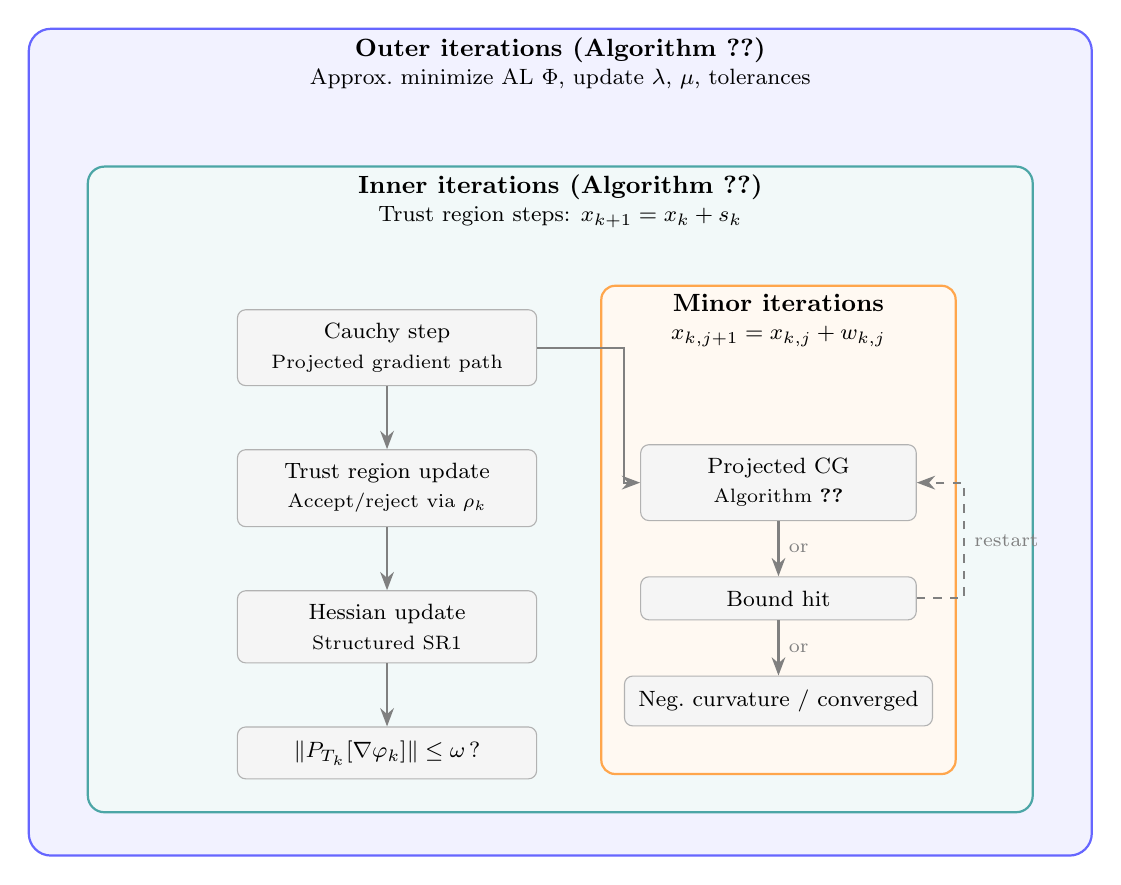
\begin{tikzpicture}[
		>=Stealth,
		every node/.style={font=\small},
		outerbox/.style={draw=blue!60, fill=blue!5, rounded corners=8pt, thick, inner sep=10pt},
		innerbox/.style={draw=teal!70, fill=teal!5, rounded corners=6pt, thick, inner sep=8pt},
		minorbox/.style={draw=orange!70, fill=orange!5, rounded corners=5pt, thick, inner sep=6pt},
		stepbox/.style={draw=gray!60, fill=gray!8, rounded corners=3pt, inner sep=5pt, align=center, font=\footnotesize},
		]
		% Outer iteration frame
		\node[outerbox, minimum width=13.5cm, minimum height=10.5cm, label={[font=\small\bfseries, anchor=north]north:Outer iterations (Algorithm~\ref{algo:traulls})}] (outer) {};
		\node[font=\footnotesize, anchor=north] at ([yshift=-4mm]outer.north) {Approx.\ minimize AL $\Phi$, update $\lambda$, $\mu$, tolerances};
		
		% Inner iteration frame
		\node[innerbox, minimum width=12cm, minimum height=8.2cm, label={[font=\small\bfseries, anchor=north]north:Inner iterations (Algorithm~\ref{algo:trinner_iteration})}] (inner) at ([yshift=-6mm]outer.center) {};
		\node[font=\footnotesize, anchor=north] at ([yshift=-4mm]inner.north) {Trust region steps: $x_{k+1}=x_k+s_k$};
		
		% Left column: Cauchy + TR update + Hessian update + convergence check
		\node[stepbox, minimum width=3.8cm] (cauchy) at ([xshift=-2.2cm, yshift=1.8cm]inner.center) {Cauchy step\\[1pt]{\scriptsize Projected gradient path}};
		\node[stepbox, minimum width=3.8cm, below=8mm of cauchy] (trupdate) {Trust region update\\[1pt]{\scriptsize Accept/reject via $\rho_k$}};
		\node[stepbox, minimum width=3.8cm, below=8mm of trupdate] (hessupdate) {Hessian update\\[1pt]{\scriptsize Structured SR1}};
		\node[stepbox, minimum width=3.8cm, below=8mm of hessupdate] (convcheck) {$\|P_{T_k}[\nabla\varphi_k]\| \le \omega$\,?};
		
		% Minor iteration frame
		\node[minorbox, minimum width=4.5cm, minimum height=6.2cm, right=8mm of cauchy, anchor=north west, yshift=8mm, label={[font=\small\bfseries, anchor=north]north:Minor iterations}] (minor) {};
		\node[font=\footnotesize, anchor=north] at ([yshift=-4mm]minor.north) {$x_{k,j+1}=x_{k,j}+w_{k,j}$};
		
		% Inside minor: PCG + termination
		\node[stepbox, minimum width=3.5cm] (pcg) at ([yshift=6mm]minor.center) {Projected CG\\[1pt]{\scriptsize Algorithm~\ref{algo:projected_cg_method}}};
		\node[stepbox, minimum width=3.5cm, below=7mm of pcg] (boundhit) {Bound hit};
		\node[stepbox, minimum width=3.5cm, below=7mm of boundhit] (negcurv) {Neg.\ curvature / converged};
		
		% Arrows left column
		\draw[->, thick, gray] (cauchy) -- (trupdate);
		\draw[->, thick, gray] (trupdate) -- (hessupdate);
		\draw[->, thick, gray] (hessupdate) -- (convcheck);
		
		% Arrow Cauchy -> minor
		\draw[->, thick, gray] (cauchy.east) -- ([xshift=-2mm]pcg.west|-cauchy.east) -- ([xshift=-2mm]pcg.west) -- (pcg.west);
		
		% Arrows inside minor
		\draw[->, thick, gray] (pcg) -- node[right, font=\scriptsize]{or} (boundhit);
		\draw[->, thick, gray] (boundhit) -- node[right, font=\scriptsize]{or} (negcurv);
		
		% Restart loop for bound hit
		\draw[->, thick, gray, dashed] (boundhit.east) -- ++(6mm,0) |- node[right, font=\scriptsize, pos=0.25]{restart} (pcg.east);
		
	\end{tikzpicture}
	\caption{Hierarchy of the three iteration levels in the AL algorithm. The outer loop updates the Lagrange multipliers and penalty parameter. Each outer iteration triggers a sequence of trust-region inner iterations, and each inner iteration computes its step via a Cauchy point followed by minor iterations using the projected conjugate gradient method.}
	\label{fig:iteration_hierarchy}
\end{figure}
Our intention with the work presented in this paper was to conceive an algorithm able to handle directly linear constraints of the form~\eqref{eq:linear_constraints} but we also accept problems where linear constraints are only bounds and then
\[\Omega = \left\{x \in \RR^n \ |\ l \le x \le u\right\}.\]
The framework we have presented remains valid for this formulation. The only practical difference is in the computation of projections. In the bound constrained  case, the projection of a vector $x$ on the set $\Omega$ has components
\begin{equation}\label{eq:projection_bounds}
	\left(\proj{\Omega}{x}\right)_i = 
	\left\{ \begin{aligned}
		& l_i & &\text{if } x_i < l_i \\
		& x_i & &\text{if } x_i \in [l_i,u_i] \\
		& u_i & &\text{if } x_i > u_i
	\end{aligned} \right.
\end{equation}
In our implementation, the only practical difference with the polyhedral case is that we can use directly the norm of the projected gradient
\[\left\| x_K - \proj{\Omega}{x_K-\nabla_x\Phi_K}\right\|,\]
as a criticality measure.

The default values for tolerances and constants of Algorithm~\ref{algo:traulls} are
\[ \mu_0 = 10,\ \kappa_\omega = \beta_\omega = \eta = \omega = 1,\ \kappa_\eta = 0.1,\ \beta_\eta = 0.9,\ \tau = 100,\  \omega_*=\eta_* = 10^{-7}.\]
The constants relative to the inner minimization process of Algorithm~\ref{algo:trinner_iteration} are set to the subproblem criticality tolerance, i.e. at outer iteration $K$, we set
\[ \kappa_{cg} = \kappa_{mlt} = \omega_K.\]
The value of constant $\kappa_{sds}$ used safeguard~\eqref{eq:structured_sr1_safeguard} is set to the square root of the relative double precision.

At the start of each outer iteration, we set our initial approximation of the second order terms of the Hessian to $B_0 = 0$ and the constant used to monitor the hybrid switching scheme~\eqref{eq:hybrid_update_strategy} of the Hessian is set to $\kappa_{hyb}=0.1$.

We now discuss the trust region handling. The initial radius value for Algorithm~\ref{algo:trinner_iteration} is set to
\begin{equation*}
	\Delta_0 = 0.1\| g_0\|_\infty.
\end{equation*}
The mechanism to update the trust region given in~\eqref{eq:tr_basic_update} still leaves important flexibility. We choose to follow a standard strategy similar to the one exposed in~\cite[][Chapter 17]{conn-etal:2000}. We also added a refinement to handle the case where the ratio $\rho_k$ is negative, which can happen when there is very poor agreement between the function and the model. In such cases, we reduce more severely the radius by taking
\[\Delta_{k+1} = \gamma_1 \Delta_k.\]
The complete update rule for the trust region radius is then
\begin{equation*}
	\Delta_{k+1} = \left\{\begin{aligned}
		& \max\left(\alpha_2 \|s_k\|_\infty,\Delta_k\right) & &\text{if } \rho_k \ge \eta_2 \\
		& \Delta_k &  &\text{if } \rho_k \in [\eta_1,\eta_2) \\
		& \alpha_1\|s_k\|_\infty & &\text{if } \rho_k \in [0,\eta_1) \\
		& \min\left(\alpha_1 \|s_k\|_\infty,\gamma_1\Delta_k\right) & &\text{if } \rho_k < 0,
	\end{aligned}\right.
\end{equation*}
with constant values
\[\alpha_1 = 0.25,\ \alpha_2 = 2.5,\ \eta_1 = 0.25,\ \eta_2 = 0.75,\ \gamma_1 = 0.0625.\]


\section{Convergence analysis}\label{sec:convergence_analysis}

In this section, we study the convergence of Algorithm~\ref{algo:traulls} towards a first-order critical point of problem~\eqref{pb:cnls}. We start by showing global convergence of Algorithm~\ref{algo:trinner_iteration}, implying that the inner minimization phase of Algorithm~\ref{algo:traulls} is always well defined. We then establish global convergence of the main algorithm. Our analysis is based on the criticality measure, i.e. the norm of the projected gradient, which differs from the reduced gradient norm~\eqref{eq:criticality_cond_reduced_grad} used in our implementation. At the end of this section, we discuss the validity of our convergence results when~\eqref{eq:criticality_cond_reduced_grad} is used as a inner iteration termination condition instead of~\eqref{eq:crit_norm_projected_grad}.

\subsection{Global convergence of the inner minimization}

Because our inner-minimization procedure closely resembles the SBMIN algorithm~\cite{conn-etal:1988b} -- used in the bound-constrained inner-minimization phase of LANCELOT~\cite{conn-etal:1992} -- our proof follows the structure of the global convergence proof in~\cite{conn-etal:1988a}. Most of the work lies in reformulating and adapting the intermediate results to the polyhedral case, accounting for the structure of the linear constraints.

We first make the standard assumption
\begin{assumption}\label{assumption:inner_iterates_compact}
	The set $\calX = \left\{x \ | \ \varphi(x) \le \varphi(x_0)\right\} \cap \Omega$ is non empty and compact.
\end{assumption}
By Assumption~\ref{assumption:functions_C2}, it is implicit that the function $\varphi$ is twice continuously differentiable on $\calX$ so we will not state this in the propositions given in this section.

We remind that the quadratic model is of the form
\[q_k(s) = \dfrac{1}{2} \inner{s}{H_ks} + \inner{g_k}{s},\]
where $g_k = \nabla \varphi(x_k)$ and $H_k$ is an approximation of the Hessian based on the structured SR1 formula from~\ref{subsec:hessian_approx}. We formulate two assumptions relative to those approximations. The norm used is the induced norm on matrices, i.e. $\|M\| := \sup_{\|x\|=1} \|Mx\|$ for a given matrix $M$.
\begin{assumption}\label{assumption:model_hessian}
	Defining, for every iteration index $k$, the scalars $b_k$ by 
	\[b_k = 1+\max_{0 \le i \le k} \ \left\| H_i\right\|,\]
	we require that the series $\sum_k \frac{1}{b_k}$ diverges to $\infty$.
\end{assumption}
The second assumption states that the norm of the approximating Hessians should not increase too fast compared with the speed of convergence of the function values.
\begin{assumption}\label{assumption:hessian_norm_compared_convergence_speed}
	\[\lim\limits_{k\to \infty} b_k (\varphi_{k+1}-\varphi_k) = 0.\]
\end{assumption}

The projected gradient path is defined as
\[s_k(t)=\proj{\Omega}{x_k-tg_k}-x_k \text{ for } t\ge 0.\]
The reduction of the model along the projected gradient path may thus be defined as the piecewise quadratic function
\[\psi(t) = q_k(s_k(t)),\]
and we denote by $t_k^C$ the first local minimum of $\psi$ subject to the trust region constraint 
\begin{equation*}
	\|s_k(t)\|_\infty \le \Delta_k.
\end{equation*}
The associated Cauchy step is 
\begin{equation*}
	s_k^C = s_k(t_k^C).
\end{equation*}
Because of the choice of the $\ell_\infty$ norm, computing $s_k(t)$ within the trust region corresponds to project the direction $x_k-tg_k$ onto
\begin{equation}\label{eq:proj_grad_feasible_set}
	\left\{d \in \RR^n \ | \ Ad=0,\ l_k \le d \le u_k\right\},
\end{equation}
with $(l_k)_i = \max\left(-\Delta_k,l_i-(x_k)_i\right)$ and $(u_k)_i = \min\left(\Delta_k,u_i-(x_k)_i\right)$ for all $i=1,\ldots,n$.

We assume that the total step $s_k$ produces a fraction of the reduction achieved by the Cauchy point:
\begin{equation}\label{eq:step_drecrease_wrt_cauchy}
	q_k(s_k) \le \kappa_{fcd} \ q_k(s_k^C),
\end{equation}
for $\kappa_{fcd} \in (0,1]$. 

We detail the behavior of the polygonal line $s_k(t)$. Let $I(t)$ be the set of bounds $l_k$ or $u_k$ satisfied with equality at $s_k(t)$. Notice that this definition slightly differs from the active set $I(x)$ defined earlier, as the new formulation know takes into account the trust region. At first, if no bounds are active at $x_k$, projecting on the set~\eqref{eq:proj_grad_feasible_set} for $t$ close to $0$ is equivalent to projecting onto the null space of $A$. As $t$ increases, the direction might hit several bounds. Since the set of active bounds can only be increased, we have that
\begin{equation}\label{eq:nested_active_sets}
	I(t) \subseteq I(t^\prime) \quad \text{for all}\ 0 < t \le t^\prime.
\end{equation}
Let \(0=t_0 < t_1 < \ldots < t_p\) be the successive values of $t$ at which the projected step $s_k(t)$ hits a bound, also called breakpoints. Hitting a bound not only affects the corresponding components, that are now fixed, but it also affects the other components, as the steepest direction must now be projected on a subspace
\[\left\{d \in \RR^n \ | \ Ad=0,\ d_i=0\ \text{fixed components}\ i\right\}\]
This motivates to adapt the notion of tangent space at a point on the projected gradient path:
\begin{equation*}
	T(t) := \left\{ d \in \RR^n \ | \ Ad = 0,\ d_i=0\ \text{for all}\ i\in I(t)\right\},
\end{equation*}
for $t\ge0$. This enables us to give a recursive expression of $s_k(t)$ on each interval $[t_i,t_{i+1})$, with $0 \leq i \le p$, as:
\begin{equation}\label{eq:projected_gradient_path_recursion}
	s_k(t) = (t-t_i) \proj{T(t_i)}{-g_k} + s_k(t_i).
\end{equation}
We also define the reduced gradient on the projected gradient path:
\begin{equation}\label{eq:reduced_gradient_proj_grad_path}
	z_k(t) := \proj{T(t)}{g_k}.
\end{equation}
Note that the reduced gradient, and hence the path $s_k(t)$ are well defined because of the full rank Assumption~\ref{assumption:full_rank_A} of the matrix $A$. As for the differentiability of $\varphi$, we will not remind it in the results of this section.

We now state a first lemma on how the tangent spaces and the reduced gradients at two different positions compare to each other.
\begin{lemma}\label{lemma:non_increasing_reduced_gradient_norm}
	For all $0 < t < t^\prime$, we have that 
	\begin{equation*}
		T(t) \supseteq T(t^\prime),
	\end{equation*}
	and
	\begin{equation}\label{eq:lemma_reduced_gradient_norm}
		\|z_k(t)\| \ge \|z_k(t^\prime)\|.
	\end{equation}
\end{lemma}
\begin{proof}
	The first statement follows from the inclusion~\eqref{eq:nested_active_sets}. Inequality~\eqref{eq:lemma_reduced_gradient_norm} then results from the fact that projecting the same vector on a smaller linear subspace reduces the norm of its projection. 
\end{proof}
When referring to the tangent space and the reduced gradient at a given breakpoint $t_i$, we will make use of the shorthand notation $T_i := T(t_i)$ and $z_i:=z_k(t_i)$. Notice that because the active set is fixed on each interval $[t_i,t_{i+1})$, so is the tangent space and hence, the reduced gradient is constant. Also, we can deduce from Lemma~\ref{lemma:non_increasing_reduced_gradient_norm} that the tangent spaces associated to each breakpoint form a finite sequence of nested linear subspaces
\[T_0 \supseteq T_1 \supseteq \ldots \supseteq T_p.\]
We can now expand equation~\eqref{eq:projected_gradient_path_recursion}:
\begin{equation}\label{eq:projected_gradient_path_full_expr}
	s_k(t) = -(t-t_i)z_i - \sum_{j=0}^{i-1}(t_{j+1}-t_j)z_j,
\end{equation}
which shows that on each interval $(t_i,t_{i+1})$, $s_k(t)$ is differentiable w.r.t. $t$ and that
\begin{equation}\label{eq:projected_gradient_path_derivative}
	s_k^\prime(t) = -z_k(t) = -z_i,
\end{equation}
for $t \in (t_i,t_{i+1})$.

We start by establishing an inequality on the decrease of the objective function after taking step $s_k$. This will involve the norm of the projected gradient, i.e.:
\begin{equation}\label{eq:crit_norm_projected_grad}
	h_k := \left\|s_k(1)\right\|.
\end{equation}

\begin{lemma}\label{lemma:majoration_reduced_gradient_norm}
	If Assumption~\ref{assumption:inner_iterates_compact} holds and that $h_k>0$, then 
	\[\|z_k(t_k^{(1)})\| \ge \dfrac{h_k}{2},\]
	where \[t_k^{(1)}=\frac{h_k}{2\kappa_{ubg}},\]
	and $\kappa_{ubg}$ is the constant defined by $\kappa_{ubg} := \max\left(1, \max_{x \in \calX} \|\nabla \varphi(x)\|\right)$.
\end{lemma}

\begin{proof} 
	First note that the constant $\kappa_{ubg}$ is well defined because $\varphi$ is continuously differentiable on $\calX$, the latter being compact by Assumption~\ref{assumption:inner_iterates_compact}.
	
	Since the set $\Omega$ is closed and convex, the projection mapping $\proj{\Omega}{\cdot}$ is non expansive, thus, for any $t\ge 0$:
	\begin{equation*}
		\begin{split}
			\left\| s_k\left(t\right) \right\| & = \left\| \proj{\Omega}{x_k-tg_k}-x_k\right\| \\
			& = \left\| \proj{\Omega}{x_k-tg_k}-\proj{\Omega}{x_k}\right\| \\
			& \le \left\| x_k-tg_k-x_k\right\|\\
			& \le t\|g_k\|.
		\end{split}
	\end{equation*}
	Choosing $t=t_k^{(1)}$ and because $\|g_k\|\le \kappa_{ubg}$ by definition of $\kappa_{ubg}$, we get
	\begin{equation}\label{eq:norm_proj_grad_t1}
		\| s_k(t_k^{(1)})\| \le \dfrac{h_k}{2}.
	\end{equation}
	Now, defined $t_k^{(2)}$ as the smallest $t\ge 0$ such that
	\begin{equation}\label{eq:def_t2}
		\|s_k(t_k^{(2)})\| = h_k.
	\end{equation}
	By~\eqref{eq:norm_proj_grad_t1}, we have
	\begin{equation}\label{eq:t1_leq_t2}
		0 < t_k^{(1)} < t_k^{(2)} \le 1.
	\end{equation}
	On each interval $(t_i,t_{i+1})$, the left, resp. right, derivative of $s_k(t)$ at $t_i$, resp. $t_{i+1}$, are well defined and equal $z_i$. We can thus rewrite~\eqref{eq:projected_gradient_path_full_expr} as
	\begin{equation*}
		s_k(t) = \int_{t_i}^{t} s_k^\prime(t)dt + \sum_{j=0}^{i-1} \int_{t_j}^{t_{j+1}} s_k^\prime(t)dt,
	\end{equation*} 
	which we simplify by
	\begin{equation}\label{eq:projected_gradient_path_integral_form}
		s_k(t) = -\int_{0}^{t} z_k(t)dt,
	\end{equation}
	using~\eqref{eq:projected_gradient_path_derivative} and keeping in mind that it is a sum of integrals defined on each segment $[t_i,t_{i+1}]$. 
	Now let $i_1$, resp. $i_2$ be the breakpoint index such that $t_k^{(1)} \in [t_{i_1},t_{i_1+1})$, resp. $t_k^{(2)} \in [t_{i_2},t_{i_2+1})$. Then by~\eqref{eq:projected_gradient_path_integral_form}:
	\begin{equation*}
		s_k(t_k^{(2)}) - s_k(t_k^{(1)}) = -\int_{t_k^{(1)}}^{t_k^{(2)}} z_k(t)dt, 
	\end{equation*}
	which leads to
	\begin{equation*}
		\begin{split}
			\|s_k(t_k^{(2)}) - s_k(t_k^{(1)})\| & \le \int_{t_k^{(1)}}^{t_k^{(2)}} \|z_k(t)\|dt \\
			& \le \int_{t_k^{(1)}}^{t_k^{(2)}} \|z_k(t_k^{(1)})\|dt \\
			& \le (t_k^{(2)}-t_k^{(1)}) \|z_k(t_k^{(1)})\|,
		\end{split}
	\end{equation*}
	where we have used~\eqref{eq:lemma_reduced_gradient_norm} to bound the norm of the reduced gradient on $[t_k^{(1)},t_k^{(2)}]$.
	Combined with~\eqref{eq:t1_leq_t2} and~\eqref{eq:def_t2}, we get
	\begin{equation*}
		\begin{split}
			\dfrac{h_k}{2} = \|s_k(t_k^{(2)})\| - \dfrac{h_k}{2} &\le  \|s_k(t_k^{(2)})\| - \|s_k(t_k^{(1)})\| \\ 
			& \le \|s_k(t_k^{(2)}) - s_k(t_k^{(1)})\| \\
			& \le 	(t_k^{(2)}-t_k^{(1)}) \|z_k(t_k^{(1)})\| \\
			& \le  \|z_k(t_k^{(1)})\|,
		\end{split}
	\end{equation*}
	which is the desired inequality.
\end{proof}

The next lemma gives an upper bound on the quadratic model $\psi(t)$ in an interval of interest.

\begin{lemma}\label{lemma:bound_model_proj_grad_path}
	If Assumption~\ref{assumption:inner_iterates_compact} holds and that for some $t_k^{(3)}>0 $, one has
	\[\alpha_k = \|z_k(t_k^{(3)})\| > 0,\]
	then, if $T$ is the set of points in $[0,t_k^{(3)}]$ at which the piecewise quadratic $\psi$ is differentiable, 
	\begin{equation}\label{eq:lemma_ineq_model_derivative_t3}
		\psi^\prime(t) \le -\alpha_k^2 + t_k^{(3)}\kappa_{ubg}^2\|H_k\|,
	\end{equation}
	for all $t\in T$.
	
	Furthermore, 
	\begin{equation*}
		\psi^\prime(t) \le -\dfrac{1}{2}\alpha_k^2 ,
	\end{equation*}
	for all $t\in T \cap [0,t_k^{(4)}]$ and 
	\begin{equation*}
		\psi(t) \le  - \dfrac{\alpha_k^2}{2}t,
	\end{equation*}
	for all $t\in  [0,t_k^{(4)}]$ where 
	\begin{equation}\label{eq:t4_def}
		t_k^{(4)} = \min \left(t_k^{(3)}, \dfrac{\alpha_k^2}{2\kappa_{ubg}^2(\|H_k\|+1)}\right).
	\end{equation}
\end{lemma}

\begin{proof}
	For $t \in T$, let $i$ be the breakpoint index such that $t\in(t_i,t_{i+1})$. On the latter interval, $\psi$ is differentiable and we have, by expression~\eqref{eq:projected_gradient_path_full_expr}:
	\begin{equation*}
		\begin{split}
			\psi^\prime(t) & = \inner{g_k}{s_k^\prime(t)} + \inner{s_k(t)}{H_ks_k^\prime(t)} \\
			& = -\inner{g_k}{z_i} - \inner{s_k(t)}{H_kz_i}.
		\end{split}
	\end{equation*}
	Because $z_i$ is, by definition, the orthogonal projection of the vector $g_k$ on a linear subspace:
	\begin{equation}\label{eq:ineq_derivative_model_first_order}
		\begin{split}
			\inner{g_k}{z_i} & = \inner{z_i}{z_i} \\
			& \ge \|z_k(t_k^{(3)})\|^2 = \alpha_k^2,
		\end{split}
	\end{equation}
	where the last inequality follows from the monotonicity of the reduced gradient norm on $[0,\infty)$. 
	
	We now look at the quadratic terms. First, by Cauchy-Schwarz inequality:
	\begin{equation*}
		\left|\inner{s_k(t)}{H_kz_i}\right| \le \|s_k(t)\| \|H_kz_i\|.
	\end{equation*}
	Then, applying the triangle inequality to expression~\eqref{eq:projected_gradient_path_full_expr}, we obtain
	\begin{equation}\label{eq:norm_proj_grad_step_ineq}
		\begin{split}
			\|s_k(t)\| & \le (t-t_i) \|z_i\| + \sum_{j=0}^{i-1} (t_{j+1}-t_j)\|z_j\| \\
			& \le (t-t_i) \|g_k\| + \sum_{j=0}^{i-1} (t_{j+1}-t_j)\|g_k\| \\
			& \le t\|g_k\| \le t_k^{(3)}\kappa_{ubg},
		\end{split}
	\end{equation}
	where we have used the facts that for all breakpoints indices $j$, $\|z_i\| \le \|g_k\| \le \kappa_{ubg}$ and that the scalar $t$ is taken in $T$. For the remaining terms:
	\begin{equation*}
		\|H_kz_i\| \le \|H_k\| \|z_i\| \le \kappa_{ubg}\|H_k\|.
	\end{equation*}
	Combining the latter inequality with~\eqref{eq:norm_proj_grad_step_ineq}, we get the following bound for the quadratic terms:
	\begin{equation}\label{eq:ineq_derivative_model_second_order}
		\left|\inner{s_k(t)}{H_kz_i}\right| \le t_k^{(3)} \kappa_{ubg}^2 \|H_k\|.
	\end{equation}
	Hence, using~\eqref{eq:ineq_derivative_model_first_order} and~\eqref{eq:ineq_derivative_model_second_order}:
	\begin{equation*}
		\psi^\prime(t) \le -\alpha_k^2 + t_k^{(3)} \kappa_{ubg}^2 \|H_k\|,
	\end{equation*}
	for all $t \in T$, which proves~\eqref{eq:lemma_ineq_model_derivative_t3}.
	Now, considering $t_k^{(4)}$ as defined by~\eqref{eq:t4_def}, since $t_k^{(4)} \le t_k^{(3)}$, we get that $\|z_k(t_k^{(4)})\| \ge \alpha_k > 0$. The above reasoning based on $t_k^{(4)}$ thus yields
	\begin{equation*}
		\psi^\prime(t) \le -\alpha_k^2 + t_k^{(4)} \kappa_{ubg}^2 \|H_k\| \le -\dfrac{\alpha_k^2}{2},
	\end{equation*}
	for $t\in T$, $t\le t_k^{(4)}$. It follows that, for all $t\in [0,t_k^{(4)}]$:
	\begin{equation*}
		\psi(t) \le -\dfrac{\alpha_k^2}{2}t,
	\end{equation*}
	which completes the proof.
\end{proof}

We can now establish a bound on the decrease guaranteed by the step.
\begin{theorem}
	If assumptions~\ref{assumption:inner_iterates_compact}, \ref{assumption:model_hessian} hold and that $h_k > 0$, then
	\begin{equation}\label{eq:bound_step_decrease}
		q_k(s_k) \le -\kappa_{mdc} h_k^2 \min\left(\dfrac{h_k^2}{b_k},\Delta_k\right),
	\end{equation}
	where 
	\begin{equation*}
		\kappa_{mdc} = \dfrac{\kappa_{fcd}}{64\kappa_{ubg}^2}.
	\end{equation*}
	Furthermore, if iteration $k$ is successful, then
	\begin{equation}\label{eq:bound_successful_step_decrease}
		\varphi(x_k) - \varphi(x_k+s_k) \ge \kappa_{sdc} h_k^2 \min\left(\dfrac{h_k^2}{b_k},\Delta_k\right),
	\end{equation}
	with $\kappa_{sdc} = \eta_1 \kappa_{mdc}$.
\end{theorem} 
\begin{proof}
	We first observe that if we use $t_k^{(1)}$ as $t_k^{(3)}$ in the proof of Lemma~\ref{lemma:bound_model_proj_grad_path} and apply Lemma~\ref{lemma:majoration_reduced_gradient_norm}, we get 
	\begin{equation}\label{eq:model_bound_t1}
		\psi(t) \le -\dfrac{h_k^2}{8} t,
	\end{equation}
	for $t \in [0,t_k^{(5)}]$ with \[t_k^{(5)} := \min\left(t_k^{(1)},\dfrac{h_k^2}{8\kappa_{ubg}^2 (\|H_k\|+1)}\right) = \dfrac{h_k^2}{8\kappa_{ubg}^2 (\|H_k\|+1)}.\]
	We will bound the decrease obtained with the step depending on where the point associated with $t_k^{(5)}$ lies with respect to the trust region boundary.
	
	First, assume that $\|s_k(t_k^{(5)})\|_\infty \le \Delta_k$. By~\eqref{eq:model_bound_t1}, one has $\psi^\prime(t) < -h_k^2 /8 < 0$ for all $t \in  [0,t_k^{(5)}]$, so $\psi$ in strictly decreasing on this segment. Because the Cauchy point is the first local minimizer of $\psi$ subject to the trust region and the trust region is not violated at $t_k^{(5)}$, we must have $t_k^C \ge t_k^{(5)}$. Therefore, 
	\[\psi(t_k^C) \le \psi(t_k^{(5)}) \le -\dfrac{h_k^2}{8} t_k^{(5)} \]
	
	Then, by~\eqref{eq:step_drecrease_wrt_cauchy}, $q_k(s_k) \le \kappa_{fcd} q_k(s_k^C)$ and it follows that
	\begin{equation}\label{eq:model_decrease_cauchy_in_tr}
		q_k(s_k) \le -\kappa_{fcd} \frac{h_k^2}{8} t_k^{(5)}.
	\end{equation}
	Now, assume that $\|s_k(t_k^{(5)})\|_\infty > \Delta_k$. The latter implies that $\|s_k(t_k^C)\|_\infty = \Delta_k$ and from
	\begin{equation*}
		\left\|s_k\left(\frac{\Delta_k}{\kappa_{ubg}}\right)\right\|_\infty \le 	\left\|s_k\left(\frac{\Delta_k}{\kappa_{ubg}}\right)\right\| \le \frac{\Delta_k}{\kappa_{ubg}} \|g_k\| \le \Delta_k,
	\end{equation*}
	we can deduce that 
	\begin{equation*}
		t_k^C \ge \frac{\Delta_k}{\kappa_{ubg}}.
	\end{equation*}
	Therefore, using~\eqref{eq:model_bound_t1} with $t=t_k^C$ and~\eqref{eq:step_drecrease_wrt_cauchy} implies
	\begin{equation}\label{eq:model_decrease_cauchy_at_tr}
		q_k(s_k) \le -\kappa_{fcd} \frac{h_k^2}{8\kappa_{ubg}} \Delta_k \le -\kappa_{fcd} \frac{h_k^2}{64\kappa_{ubg}^2} \Delta_k,
	\end{equation} 
	because $\kappa_{ubg} \ge 1.$
	The inequality~\eqref{eq:bound_step_decrease} results from gathering~\eqref{eq:model_decrease_cauchy_in_tr},~\eqref{eq:model_decrease_cauchy_at_tr} and the definition of scalar $b_k$. 
	
	Finally, if the step is successful, we get inequality~\eqref{eq:bound_successful_step_decrease} by using~\eqref{eq:bound_step_decrease} and the step acceptance condition $\rho_k > \eta_1$ from Algorithm~\ref{algo:trinner_iteration}. 
\end{proof}

Once we have established the guaranteed decrease inequality~\eqref{eq:bound_step_decrease}, the rest of the proof does not involve the polyhedral structure of the constraints and we can fall back into the standard convergence theory of trust region methods. We state the main convergence theorem, whose proof and intermediate developments can be found in~\cite{conn-etal:1988a}.
\begin{theorem}[Theorem 11 from~\cite{conn-etal:1988a}]
	If assumptions~\ref{assumption:inner_iterates_compact}, \ref{assumption:model_hessian}, \ref{assumption:hessian_norm_compared_convergence_speed} hold, then
	\[\lim\limits_{k\to \infty} h_k = 0.\]
\end{theorem}

\subsection{Global convergence of the algorithm}

The content of this section follows the structure of the global convergence proof outlined in~\cite{conn-etal:1996b} for AL algorithms designed to solve problems whose constraints combine nonlinear equalities and linear inequalities. We first make the following assumption about the iterates considered.

\begin{assumption}\label{assumption:iterates_domain_bounded}
	The iterates produced by Algorithm~\ref{algo:traulls} lie within a closed bounded domain of $\Real^n$.
\end{assumption}

Let $(x_k)_k$ be a sequence of such iterates, then Assumption~\ref{assumption:iterates_domain_bounded} ensures the existence of a subsequence indexed by $\calK \subseteq \NN$ converging to a limit point $x_*$. Since the iterates satisfy $x_k \in \Omega$ for all $k$, we also have $x_* \in \Omega$. We recall from~\eqref{eq:tangent_space} that $I(x)$ is the set of bounds active at $x$ and $T(x)$ the associated tangent space, and we abbreviate $I_* := I(x_*)$. We denote by $\tilde A_*$ the matrix gathering the linear constraints active at $x_*$,
\begin{equation*}
	\tilde A_* := \begin{pmatrix} A \\ Z_* \end{pmatrix},
\end{equation*}
where $Z_*$ is the submatrix of the identity whose rows are $e_i^\top$, $i \in I_*$. Consistently with the well-posedness of the projector~\eqref{eq:minor_subpb_projector}, $\tilde A_*$ has full row rank, so $T(x_*) = \mathrm{null}(\tilde A_*)$ and the columns of the orthonormal matrix $N_*$ form a basis of $T(x_*)$. The next assumption ensures that the null space of the active linear constraints is large enough to achieve feasibility of the nonlinear constraints, and that the gradients of those constraints are linearly independent within that space.

\begin{assumption}\label{assumption:cq_null_space_jacobian}
	The rank of the matrix $C(x_*)N_*$ is no smaller than $n_c$ at any limit point $x_*$ of the sequence $(x_k)_k$.
\end{assumption}

We now introduce the remaining notations and notions used in our convergence analysis.

Since $\Omega$ is of the form~\eqref{eq:linear_constraints}, the normal cone to $\Omega$ at $x \in \Omega$ can be defined as
\begin{equation}\label{eq:normal_cone}
	\calN_\Omega(x) = \bigg\{ A^\top\xi + \sum_{i \in I^+(x)} \sigma^+_i e_i - \sum_{i \in I^-(x)} \sigma^-_i e_i \ \Big|\ \xi\in\RR^m,\ \sigma^+_i, \sigma^-_i\ge0\bigg\},
\end{equation}
where the equality multipliers $\xi$ are free in sign while the bound multipliers are signed. The first-order criticality condition $\proj{\Omega}{x_*-\nabla_x\calL(x_*,\lambda_*)}=x_*$ of problem~\eqref{pb:cnls} is then equivalent to
\[-\nabla_x\calL(x_*,\lambda_*)\in \calN_\Omega(x_*).\]

Finally, for vectors $x$ at which the matrix $C(x)N_* N_*^\top C(x)^\top$ is non-singular, the least-squares multipliers associated with $\tilde A_*$ are defined by
\begin{equation*}
	\lambda(x) = -\big((C(x)N_*)^\dagger\big)^\top N_*^\top\nabla f(x),
\end{equation*}
where $(C(x)N_*)^\dagger = N_*^\top C(x)^\top\big(C(x)N_* N_*^\top C(x)^\top\big)^{-1}$ is the right pseudoinverse of $C(x)N_*$. When $(C(x)N_*)^\dagger $ is well defined, Assumption~\ref{assumption:functions_C2} ensures that $\lambda(x)$ is differentiable and that its Jacobian $\nabla\lambda(x)$ is bounded in a neighborhood of $x_*$ (see~\cite[Lemma 2.1]{conn-etal:1996b}).

We can now proceed with the global convergence proof, starting with a first lemma giving a bound on the reduced gradient norm.
\begin{lemma}\label{lemma:bound_proj_algrad_sol_nullspace}
	Let $\left(x_k\right)_{k\in \calK} \in \Omega$ be a sequence converging to $x_*$ and such that
	\[\left\| \proj{\Omega}{x_k - \nabla_x \Phi_k}-x_k \right\| \le \omega_k,\]
	with $\lim\limits_{k\to \infty} \omega_k = 0$. Then
	\begin{equation*}
		\left\| \proj{T(x_*)}{\nabla_x \Phi_k} \right\| \le  \omega_k,
	\end{equation*}
	for all $k\in \calK$ large enough.
\end{lemma}

\begin{proof}
	To lighten the notations, we write $v_k = \proj{\Omega}{x_k - \nabla_x \Phi_k}$ and $d_k = v_k - x_k$. We have
	\begin{equation*}
		\begin{split}
			\|v_k - x_*\| &\le \|v_k - x_k\| + \| x_k - x_*\| \\
			& \le \omega_k + \| x_k - x_*\|.
		\end{split}
	\end{equation*}
	Since, by hypothesis, $\omega_k \to 0$ and $x_k \to x_*$ for $k\in \calK$, the two terms on the right hand side converge to $0$, which implies that we also have
	\begin{equation*}
		\lim\limits_{k \in \calK} v_k = x_*.
	\end{equation*}
	Therefore, there is a threshold index $k_0$ such that all bounds inactive at $x_*$ are also inactive at $v_k$ for $k \ge k_0$. This is equivalent to $I(v_k) \subseteq I_*$ for $k\ge k_0$. We then have the reverse inclusion for the associated tangent spaces $T(x_*) \subseteq T(v_k)$, giving
	\begin{equation}\label{eq:lemma_bound_redgrad_comp_norm_tanproj}
		\left\| \proj{T(x_*)}{\nabla_x \Phi_k} \right\| \le \left\| \proj{T(v_k)}{\nabla_x \Phi_k} \right\|,
	\end{equation}
	whenever $k\in \calK$ is above the threshold index $k_0$.
	
	But recall from Section~\ref{sec:algorithm} that $T(v_k)$ is the null space of a matrix $\tilde A_k$ of the form~\eqref{eq:matrix_tangent_space}. Moreover, since $v_k$ is a projection onto a convex set, it can be characterized by
	\begin{equation*}
	x_k - \nabla_x \Phi_k - v_k = -\left(\nabla_x \Phi_k + d_k\right) \in \calN_\Omega(v_k).
	\end{equation*} 
	By the expression~\eqref{eq:normal_cone}, $\calN_\Omega(v_k)$ is trivially a subset of the row space of $\tilde A_k$ and the latter is also the orthogonal complement of the null space of $\tilde A_k$, i.e.  $T(v_k)^\perp$. 
	Because $T(v_k)^\perp$ is a vector space:
	\[\nabla_x \Phi_k + d_k \in T(v_k)^\perp,\]
	and we obtain, by linearity of $\proj{T(v_k)}{\cdot}$:
	\begin{equation}\label{eq:lemma_bound_redgrad_proj_equality}
		\proj{T(v_k)}{\nabla_x \Phi_k + d_k} = 0 \iff \proj{T(v_k)}{\nabla_x \Phi_k} = -\proj{T(v_k)}{d_k}.
	\end{equation}
	Combining~\eqref{eq:lemma_bound_redgrad_comp_norm_tanproj} and~\eqref{eq:lemma_bound_redgrad_proj_equality} gives
	\begin{equation*}
		\left\| \proj{T(x_*)}{\nabla_x \Phi_k} \right\| \le \left\| \proj{T(v_k)}{\nabla_x \Phi_k} \right\| = \left\| \proj{T(v_k)}{d_k} \right\| \le \|d_k\| \le \omega_k,
	\end{equation*}
	whenever $k \in \calK$ is above the threshold $k_0$, which is the desired inequality.
\end{proof}

The next lemma is a standard result about the behavior of the Lagrange multipliers in AL methods.
\begin{lemma}[Lemma 14.4.1~\cite{conn-etal:2000}]\label{lemma:behavior_multipliers}
	Assume that $\lim\limits_{k\to \infty} \mu_k = \infty$ when Algorithm~\ref{algo:traulls} is executed. Then 
	\begin{equation*}
		\lim\limits_{k\to \infty} \frac{\|\lambda_k\|}{\mu_k} = 0.
	\end{equation*}
\end{lemma}

In the spirit of~\cite[Lemma 4.3]{conn-etal:1996b}, we state the main convergence results.
\begin{lemma}\label{lemma:key_lemma}
	Suppose that assumptions~\ref{assumption:functions_C2},~\ref{assumption:feasible_linear_cons} hold. Let $\left(x_k\right)_{k\in \calK}$ be a sequence of iterates in $\Omega$ satisfying Assumption~\ref{assumption:iterates_domain_bounded} and converging to $x_*$ for which Assumption~\ref{assumption:cq_null_space_jacobian} holds. Let $\lambda_* = \lambda(x_*)$, $(\lambda_k)_{k \in \calK}$ be any sequence of vectors and $(\mu_k)_{k \in \calK}$ be a non-decreasing sequence of positive scalars. Assume that~\eqref{eq:algo_traulls_criticality_test} holds with $\lim\limits_{k \in \calK}\omega_k = 0$.
	
	Then, there are positive constants $\kappa_2, \kappa_3$ such that
	\begin{equation}\label{eq:bound_1st_order_mult}
		\|\bar{\lambda}_k - \lambda_* \| \le \kappa_2 \omega_k + \kappa_3 \|x_k-x_*\|,
	\end{equation}
	\begin{equation}\label{eq:bound_ls_mult}
		\|\lambda(x_k) - \lambda_* \| \le \kappa_3 \|x_k-x_*\|,
	\end{equation}
	and
	\begin{equation}\label{eq:bound_norm_cons}
		\|c(x_k)\| \le \kappa_2 \frac{\omega_k}{\mu_k} + \kappa_3 \frac{\|x_k-x_*\|}{\mu_k} + \frac{\|\lambda_k - \lambda_* \|}{\mu_k}.
	\end{equation}
	If, in addition, $c(x^*) = 0$, then $x_*$ is a first-order critical point for problem~\eqref{pb:cnls} with corresponding Lagrange multipliers $\lambda_*$ and with $\lim\limits_{k \in \calK} \bar{\lambda}_k = \lim\limits_{k \in \calK} \lambda(x_k) = \lambda_*$.
\end{lemma}

\begin{proof}
	By assumptions~\ref{assumption:functions_C2} and~\ref{assumption:cq_null_space_jacobian}, for $k$ sufficiently large, the matrix $\left(C_kN_*\right)^\dagger$ is well defined, bounded and converges to $\left(C_*N_*\right)^\dagger$. Therefore, there is a constant $\kappa_2$ such that
	\begin{equation*}
		\|(\left(C_kN_*\right)^\dagger)^\top \| \le \kappa_2.
	\end{equation*}
	Furthermore, by Lemma~\ref{lemma:bound_proj_algrad_sol_nullspace}, we have
	\[ \|N_*^\top \nabla_x\Phi_k\| = \left\| \proj{T(x_*)}{\nabla_x \Phi_k} \right\| \le  \omega_k,\]
	for $k \in \calK$ large enough. Thus we may deduce
	\begin{equation}\label{eq:bound_mult_1st_ls}
		\begin{split}
			\|\bar \lambda_k - \lambda(x_k) \| & = \|(\left(C_kN_*\right)^\dagger)^\top N_*^\top\nabla f_k + \bar\lambda_k\| \\
			& = \|(\left(C_kN_*\right)^\dagger)^\top (N_*^\top\nabla f_k + (C_kN_*)^\top\bar\lambda_k)\| \\
			& = \|((C_kN_*)^\dagger)^\top (N_*^\top  \nabla_x \Phi_k)\| \\
			& \le 	\|(\left(C(x)N_*\right)^\dagger)^\top \| \ \|N_*^\top \nabla_x\Phi_k\| \\
			& \le \kappa_2 \omega_k.
		\end{split}
	\end{equation}
	Furthermore, by the mean value theorem for vector-valued functions, we have
	\[\lambda(x_k) - \lambda_* = \int_{0}^{1} \nabla \lambda(x(t))(x_k-x_*)dt,\]
	where $x(t) = x_k + t(x_*-x_k)$. The integrand is bounded for $x_k$ sufficiently close to $x_*$, hence
	\[\| \lambda(x_k) - \lambda_*\| \le \kappa_3 \|x_k-x_*\|,\]
	for $k\in \calK$ sufficiently large and for some positive constant $\kappa_3$, giving~\eqref{eq:bound_ls_mult}.
	Then, combining the latter inequality and~\eqref{eq:bound_mult_1st_ls}, we may deduce that
	\begin{equation*}
		\begin{split}
			\|\bar \lambda_k - \lambda_* \| & \le \|\bar \lambda_k - \lambda(x_k) \| + \|\lambda(x_k) - \lambda_* \| \\
			& \le \kappa_2 \omega_k + \kappa_3 \|x_k-x_*\|,
		\end{split}
	\end{equation*}
	which is inequality~\eqref{eq:bound_1st_order_mult}. 
	Next, by expression~\eqref{eq:1st_order_mult}, we have $c(x_k) = (\bar \lambda_k - \lambda_k) / \mu_k$, which leads to
	\begin{equation*}
		\begin{split}
			\|c(x_k) \| & \le \frac{\|\bar \lambda_k - \lambda_* \|}{\mu_k} + \frac{\|\lambda_k - \lambda_* \|}{\mu_k} \\
			& \le \kappa_2 \frac{\omega_k}{\mu_k} + \kappa_3 \frac{\|x_k-x_*\|}{\mu_k} + \frac{\|\lambda_k - \lambda_* \|}{\mu_k},
		\end{split}
	\end{equation*}
	where we have used~\eqref{eq:bound_1st_order_mult}.
This concludes the first part of the lemma. 
	
	Since $(\omega_k)_k$ tends to $0$ and $(x_k)_{k\in \calK}$ converges to $x_*$ by assumption, inequalities~\eqref{eq:bound_1st_order_mult} and~\eqref{eq:bound_ls_mult} imply that both sequences $(\bar \lambda_k)_k$ and $(\lambda(x_k))_k$ converge to $\lambda_*$ for $k \in \calK$. Therefore, from identity~\eqref{eq:identity_al_lag_grad}, we obtain that the sequence of gradients $\nabla_x \Phi_k$ converge to $\nabla_x \calL(x_*,\lambda_*)$. 
	
	Finally, assume that $c(x^*) = 0$. Because~\eqref{eq:algo_traulls_criticality_test} holds, we have on the one hand that 
	\begin{equation}\label{eq:norm_proj_grad_to_0}
		\lim\limits_{k \in \calK} \|\proj{\Omega}{x_k-\nabla_x \Phi_k} - x_k\|= 0.
	\end{equation}
	On the other hand, the set $\Omega$ being closed and convex, the projection mapping $\proj{\Omega}{\cdot}$ is continuous, so $\proj{\Omega}{x_k-\nabla_x \Phi_k} \to \proj{\Omega}{x_*-\nabla_x \calL(x_*,\lambda_*)}$ as $k \in \calK$ increases. With~\eqref{eq:norm_proj_grad_to_0}, we obtain
	\[\proj{\Omega}{x_*-\nabla_x \calL(x_*,\lambda_*)} = x_*.\]
	Therefore, we have established that $(x_*,\lambda_*)$ is a KKT point and the lemma is proved.
\end{proof}

We can now establish the global convergence of Algorithm~\ref{algo:traulls}.
\begin{theorem}\label{theo:global_convergence_traulls}
	Suppose that assumptions~\ref{assumption:functions_C2},~\ref{assumption:feasible_linear_cons} hold. Let $\left(x_k\right)_{k}$ be a sequence of iterates generated by Algorithm~\ref{algo:traulls} satisfying Assumption~\ref{assumption:iterates_domain_bounded}. Further assume that there is a subsequence $(x_k)_{k \in \calK}$ converging to $x_*$, for which Assumption~\ref{assumption:cq_null_space_jacobian} holds and let $\lambda_* = \lambda(x_*)$.
	Then, conclusions of Lemma~\ref{lemma:key_lemma} hold.
\end{theorem}
\begin{proof}
	As in the proof of Lemma~\eqref{lemma:key_lemma}, the inequalities~\eqref{eq:bound_1st_order_mult},~\eqref{eq:bound_ls_mult},~\eqref{eq:bound_norm_cons} can be derived from the assumptions. All that remains is to show that $c(x^*) = 0$. There are two cases to distinguish. 
	
	First, if the sequence of penalty parameters is bounded above, then there is $k$ sufficiently large such that $\|c(x_k)\| \le \eta_k$ for all $k$. Since $\eta_k \to 0$, we get that $c(x_*) = 0$.
	
	Next, if the sequence of penalty parameters is unbounded, then by the update rule, we have that $(\mu_k)_k$ grows to $\infty$. Hence, by Lemma~\ref{lemma:behavior_multipliers}, the ratio $\lambda_k /\mu_k$ converges to zero. Therefore, by inequality~\eqref{eq:bound_norm_cons}, we also obtain that $c(x_*) = 0$. 
	In both cases, $x_*$ is feasible with respect to the nonlinear constraints and the remaining conclusions of Lemma~\ref{lemma:key_lemma} hold.
\end{proof}
Our convergence analysis is based on the criticality measure~\eqref{eq:algo_traulls_criticality_test} but, as we already mentioned in Section~\ref{sec:algorithm}, the latter is not available in closed form for a general polyhedron of the form~\eqref{eq:linear_constraints}. This is what justified our choice to monitor criticality in our algorithm through the reduced gradient norm $\|P_{T(x_k)}[\nabla_x\Phi_k]\|$, which only involves the projection onto the tangent space of the currently active bounds. The two measures are linked through the tangent cone $\calT_\Omega(x_k)$, which is the dual cone of $\calN_\Omega(x_k)$. Indeed, one always has \[\|\proj{\Omega}{x_k-\nabla_x\Phi_k}-x_k\|\le\|P_{\calT_\Omega(x_k)}[-\nabla_x\Phi_k]\|\] 
and whenever the multipliers associated with the bounds active at $x_k$ are of the correct sign the projection onto the cone reduces to the projection onto $T(x_k)$, so that (see~\cite[Section 7.2]{conn-etal:1996b})
\[\|P_{\calT_\Omega(x_k)}[-\nabla_x\Phi_k]\|=\|P_{T(x_k)}[\nabla_x\Phi_k]\|.\] 
Consequently, under the assumption that these sign conditions hold at every outer iterate, the reduced-gradient rule~\eqref{eq:criticality_cond_reduced_grad} certifies the criticality test~\eqref{eq:algo_traulls_criticality_test}, and Theorem~\ref{theo:global_convergence_traulls} applies to the iterates the implementation produces. Without this assumption the reduced gradient controls only the tangential component of $\nabla_x\Phi_*$, and the limit point may not be critical.

\section{Numerical experiments}\label{sec:numerical_experiments}

In this section, we report numerical experiments conducted with the Julia implementation of our algorithm, named TRAULLS\footnote{Trust Region AUgmented nonLinear Least-squares Solver} on a Mac mini with an M4 processor and 24 GB of RAM. Our solver is open-source and can be downloaded from \url{https://github.com/UncertainLab/Traulls.jl}. All the benchmarks we present here are also accessible in the \texttt{benchmark} folder of the linked GitHub repository.
The tests were carried out on a set of 49 constrained NLS from collections~\cite{hockschittkowski:1980, schittkowski:1987, lucksanvlcek:1999} and problems 2 and 3 referenced in~\cite{biegler-etal2000}. For problems with variable dimensions, we set the number of variables to $n \in \{100, 500, 1000\}$. Thus, we have a total of 79 problem instances ranging from 2 to 1000 variables, with up to 2500 residuals and 1000 constraints. Problems with inequality constraints were converted to the form~\eqref{pb:cnls} by adding slack variables. For our tests, we set the criticality tolerance to $\omega_* = 10^{-5}$, the feasibility tolerance to $\eta_* = 10^{-6}$, the maximum number of outer iterations to 500 and the maximum number of iterations to 1000. We leave the other parameters of the algorithm at the values given at the end of Section~\ref{sec:algorithm}. We present our results with performance profiles of type~\citet{dolanmore:2002} produced with the \texttt{BenchmarkProfiles.jl} package~\cite{benchmark-profiles-julia}.

\subsection{Comparison of Hessian approximations}

Our first set of experiments compares the behavior and performance of our algorithm depending on the Hessian approximation used during the inner minimization. We compared the GN approximation~\eqref{eq:hessian_gn_approx} against structured approximations of the form~\eqref{eq:hessian_full_approx}. Based on the structured secant equation~\eqref{eq:structured_secant_eq}, we implemented the SR1 update we discussed and the BFGS update that one can derive similarly. Both structured approximations were used in their plain and hybrid variants with the switching rule~\eqref{eq:hybrid_update_strategy}.
We compared these five strategies against three metrics: computation time, number of outer iterations and number
of inner iterations. Results are indicated in Figure~\ref{fig:compare_hessians}. 
\begin{figure}[htbp]
	\centering
	\begin{subfigure}[b]{0.32\textwidth}
		\centering
		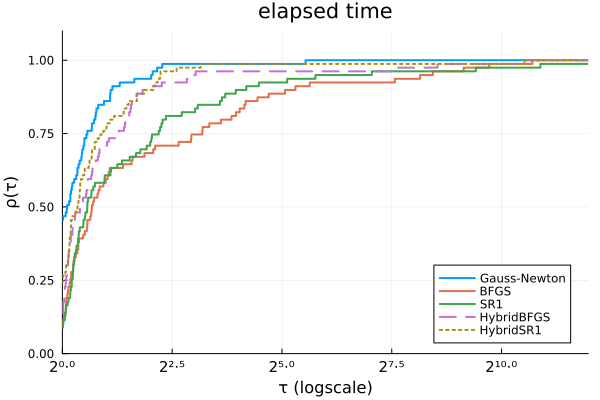
\includegraphics[width=\textwidth]{figures/traulls_all_hessians_time}
	\end{subfigure}
	\hfill
	\begin{subfigure}[b]{0.32\textwidth}
		\centering
		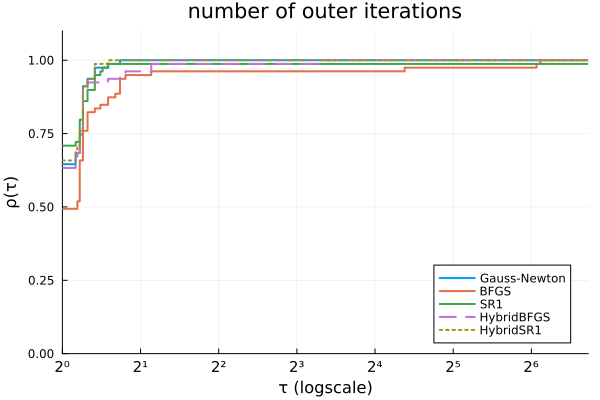
\includegraphics[width=\textwidth]{figures/traulls_all_hessians_outer}
	\end{subfigure}
	\hfill
	\begin{subfigure}[b]{0.32\textwidth}
		\centering
		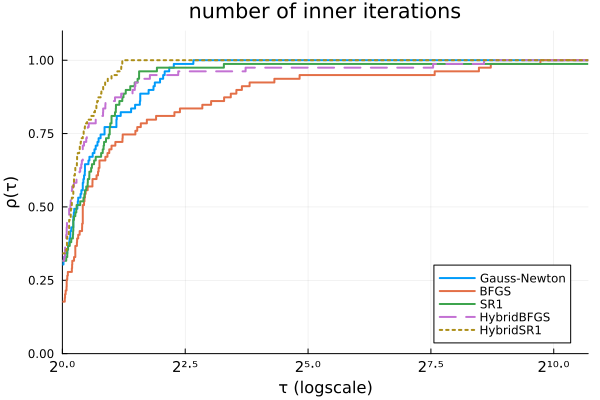
\includegraphics[width=\textwidth]{figures/traulls_all_hessians_inner}
	\end{subfigure}
	\caption{Performance profiles comparing five different Hessian approximations strategies with respect to computation time (left), number of outer iterations (center),
		and number of inner iterations (right).}
	\label{fig:compare_hessians}
\end{figure}
All five variants successfully solved all but one problem: the plain SR1 variant reaches the maximum number of iterations on the HS373 problem.
In terms of computation time, the GN approximation is the fastest: since it requires no	additional storage or update computation, it is the cheapest per iteration as our method mainly involves matrix-vector products. The GN approximation especially dominates on problems having sparse jacobians and small residuals at the solution, since the second order terms are still stored as a dense matrix. When measured by the number of inner iterations, the hybrid variants prove more efficient than their plain counterparts for both formulas. These observations are consistent with the discussion about the hybrid switching rule~\eqref{eq:hybrid_update_strategy} which -- as in the unconstrained case -- correctly identifies situations where the Gauss--Newton approximation must be corrected and activates the structured quasi-Newton correction accordingly. All approximation approaches are closer in terms of outer iterations, with plain BFGS a little bit behind, but overall, the Hybrid SR1 appears to be the most robust. To confirm these observations, we have focused our attention to a comparison of GN with Hybrid approximations, the latter appearing to be the most efficient. Profiles in Figure~\ref{fig:gn_vs_hybrid} compare the 3 approaches against the number of residual and gradient evaluations. The latter are similar to the inner iterations profile previously shown, as we evaluate the residuals one time per inner iteration and evaluate the gradient at every accepted step.
Nevertheless, Hybrid-SR1 exhibits the best efficiency and robustness. This also seems to indicate that the SR1 approximation is adequate with the negative curvature handling in the trust region setting. 
\begin{figure}[htbp]
	\centering
	\begin{subfigure}[b]{0.45\textwidth}
		\centering
		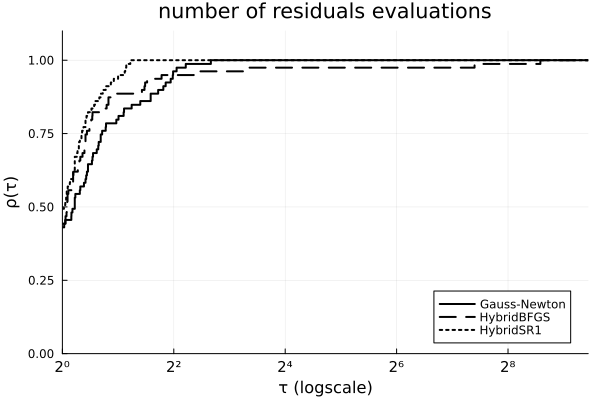
\includegraphics[width=\textwidth]{figures/gn_vs_hybrid_reseval_profile}
	\end{subfigure}
	\hfill
	\begin{subfigure}[b]{0.45\textwidth}
		\centering
		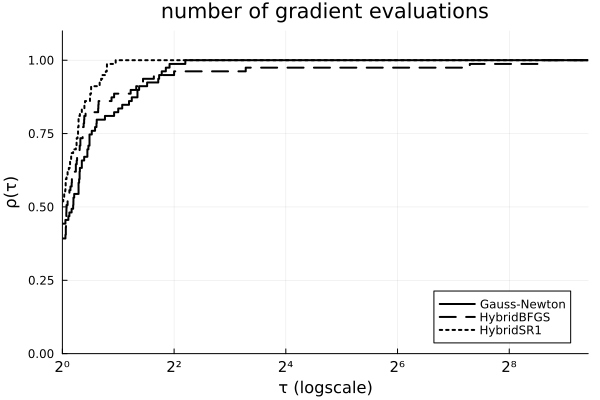
\includegraphics[width=\textwidth]{figures/gn_vs_hybrid_gradeval_profile}
	\end{subfigure}
	\caption{Performance profiles comparing the Gauss-Newton approximation against hybrid approaches with respect to the number of residual evaluations (left),
		and gradient evaluations (right).}
	\label{fig:gn_vs_hybrid}
\end{figure}
Based on these results, we retain the Hybrid SR1 variant as the best overall strategy for
TRAULLS, and use it in the comparisons that follow.

\subsection{Comparison with IPOPT and Percival}

We now compare TRAULLS (with the Hybrid SR1 approximation) against solvers IPOPT~\cite{wachterbiegler:2006} and Percival~\cite{arreckx-etal:2016}. The latter is also an augmented Lagrangian algorithm and has a native Julia implementation and uses a Julia version of the TRON~\cite{linmore:1999a} algorithm -- part of the \texttt{JSOSolvers.jl} package~\cite{migot-etal:2026} -- for the inner minimization. To benefit from the benchmarking facilities provided by the JuliaSmoothOptimizers (JSO)\footnote{https://jso.dev/} ecosystem, we used the wrapper \texttt{NLPModelsIpopt.jl}~\cite{nlp-models-ipopt-julia}. This allows us to run both solvers on our test set of problems -- all models being encoded in \texttt{NLSProblems.jl}~\cite{nls-problems-julia} -- and export the benchmark metrics using \texttt{SolverBenchmark.jl}~\cite{solver-benchmark-julia}.  To make the comparison with IPOPT relevant, we have set the parameters \texttt{nlp\_scaling\_method} = \texttt{none}, \texttt{dual\_inf\_tol} = \texttt{Inf}, \texttt{constr\_viol\_tol} = \texttt{Inf}, \texttt{compl\_inf\_tol }= \texttt{Inf}, \texttt{acceptable\_iter} = \texttt{0} and the maximum number of iterations to 1000. For Percival, since it also follows Algorithm~\ref{algo:traulls}, we have set its tolerances and parameters to the same value as ours.
For these tests, we compare the three solvers against the CPU time, the number of residual evaluations and the number of gradient evaluations. The results are presented in Figure~\ref{fig:perf_solvers}. During our experiments, IPOPT reached the maximum number of iterations on problem HS27 and returned the \texttt{unknown} internal message on problem HS70. Percival reached the maximum of iterations on the two instances of problem 5.11 from~\cite{lucksanvlcek:1999} having $n=500$ and $n=1000$.
\begin{figure}[htbp]
	\centering
	\begin{subfigure}[b]{0.32\textwidth}
		\centering
		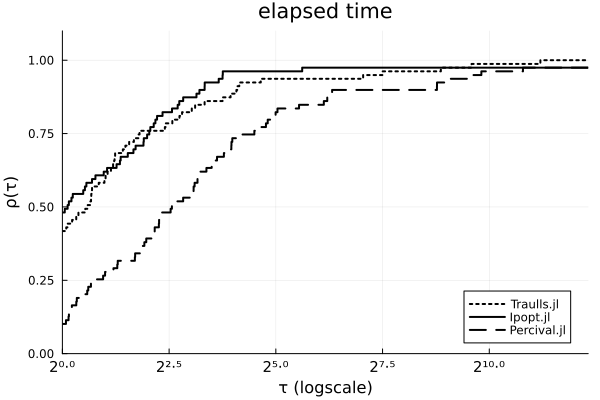
\includegraphics[width=\textwidth]{figures/traulls_vs_others_time_profile}
	\end{subfigure}
	\hfill
	\begin{subfigure}[b]{0.32\textwidth}
		\centering
		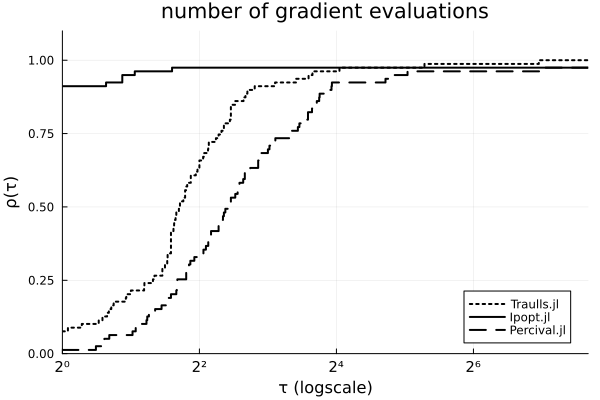
\includegraphics[width=\textwidth]{figures/traulls_vs_others_gradeval_profile}
	\end{subfigure}
	\hfill
	\begin{subfigure}[b]{0.32\textwidth}
		\centering
		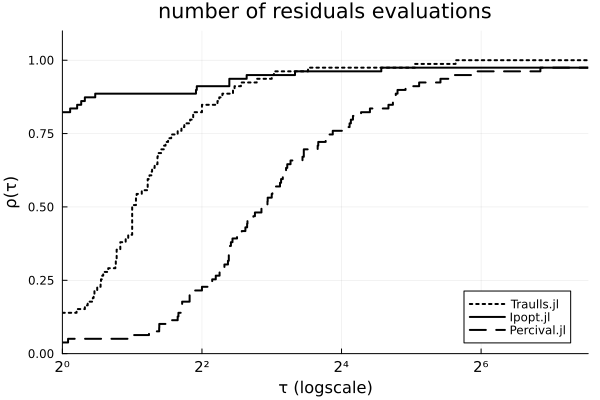
\includegraphics[width=\textwidth]{figures/traulls_vs_others_reseval_profile}
	\end{subfigure}
	\caption{Performance profiles comparing TRAULLS (Hybrid SR1), IPOPT, and Percival
		on the test set, with respect to computation time (left), residual evaluations (center),
		and gradient evaluations (right).}
	\label{fig:perf_solvers}
\end{figure}

In terms of computation time, TRAULLS and IPOPT achieve comparable performance, with
IPOPT holding a modest advantage on the fastest problems but the gap narrowing as
problem difficulty increases. Percival is consistently slower than both solvers across the
test set. Regarding the function-evaluation metrics, IPOPT dominates: its interior-point
strategy, which exploits second-order information through exact Hessians, requires
significantly fewer residual and gradient evaluations to reach convergence. TRAULLS, which
relies on a structured quasi-Newton approximation and therefore does not require exact
second derivatives, performs comparably to Percival on these metrics and outperforms it on
a majority of problems.
Across all three metrics, IPOPT is a clear winner, in spite of the two failures. However, our method is a close second in computation time and achieves similar robustness with regard to the number of residual evaluations. The clear advantage of TRAULLS over Percival shows that within the same algorithmic framework, exploiting the least-squares structures leads to better performance.
	
\section*{Conclusion}
In this paper, we have presented an algorithm able to solve NLS problems subject to constraints of general form. Our method fully exploits the structure of the problem through the AL reformulation and a structured Hessian approximation. 
Although our implementation exhibits promising performance, its limitation for large-scale applications lies in the Hessian approximation: the dense storage of the structured second order correction and the associated computations become prohibitive as the number of variables grows. A limited-memory variant of the structured update, following~\cite{byrd-etal:1994}, would be a natural extension to address this bottleneck. To tackle problems with a large number of residuals, another avenue of research could be to combine the AL framework with an adaptive sampling strategy applied to the residuals, lowering the dimensions of the inner minimization subproblems. This would extend to the constrained case techniques currently investigated for unconstrained problems~\cite{bellavia-etal:2026}.

\vspace{1em}\noindent\textbf{Acknowledgments:} The authors would like to thank Natural Sciences and Engineering Research Council of Canada (NSERC) and the Institute for Data Valorization (IVADO) in addition to Mitacs and  Hydro-Québec for their financial support through grants IT40867 and IT38322.


	


%%%%%%%%%%%%%%%% APPENDIX 
\clearpage

\section*{Appendix}

\appendix

\section{Block Cholesky factorization of the augmented Gram matrix}\label{appendix:chol_aug_matrix}
Let $A$ be an $m \times n$ full row rank matrix for which the Cholesky factor of the Gram matrix $AA^\top$ is available. Considering $\calA = \left\{i_1,\ldots, i_p\right\} \subseteq \{1,\ldots,n\}$, let $Z \in \RR^{p\times n}$ be the matrix whose row $k$ is the row $i_k$ of the $n\times n$ identity.
In this appendix, we show how to construct the Cholesky decomposition of the Gram matrix $MM^\top$, where $M$ is defined as
\[M = \begin{bmatrix}
	A \\ Z
\end{bmatrix} \in \RR^{(m+p)\times n}.\]  
Following the reasoning in~\cite[][section 4.2.9]{golubvanloan:2013} for the Cholesky decomposition of a general block matrix, we will show how, at the cost of extra computations, we can recover the Cholesky factor of $MM^\top$ using its block structure and the factor $L$. The definition of $M$ naturally leads to the block pattern
\[MM^\top = \begin{bmatrix}
	AA^\top & AZ^\top \\ ZA^\top & ZZ^\top
\end{bmatrix}\]
Simple computations first show that 
\[ZZ^\top = I_p,\quad AZ^\top = [A_{i_1},\ldots,A_{i_p}].\]
The latter, written $A_{|\calA}$, is the restriction of $A$ to the columns corresponding to the indices in $\calA$. We can write $MM^\top$ as 
\begin{equation}\label{eq:augmented_grammat}
	\begin{bmatrix}
		AA^\top &  A_{|\calA} \\  A_{|\calA}^\top & I_p
	\end{bmatrix}
\end{equation}
Let $\tilde{L}$ be $(m+p)\times(m+p)$ triangular such that $MM^\top=\tilde{L}\tilde{L}^\top$. We apply the same block structure to $\tilde{L}$, i.e.
\[\tilde{L} = \begin{bmatrix}
	\tilde{L}_{11} & 0 \\ G_{21} & \tilde{L}_{22},
\end{bmatrix},\]
with 
\begin{itemize}
	\item $\tilde{L}_{11} \ m\times m$ lower triangular
	\item $G_{21} \ p\times m$
	\item $\tilde{L}_{22} \ p \times p$ lower triangular
\end{itemize}
Verifying $MM^\top= \tilde{L}\tilde{L}^\top$ implies the matrix equality
\begin{equation}\label{eq:block_equalities_chol_fact}
	\begin{bmatrix}
		AA^\top &  A_{|\calA} \\  A_{|\calA}^\top & I_p
	\end{bmatrix}
	=
	\begin{bmatrix}
		\tilde{L}_{11}\tilde{L}_{11}^\top & \tilde{L}_{11}G_{21}^\top \\ 
		G_{21}\tilde{L}_{11}^\top & G_{21}G_{21}^\top + \tilde{L}_{22}\tilde{L}_{22}^\top
	\end{bmatrix}.
\end{equation}
By comparison of the blocks in~\eqref{eq:block_equalities_chol_fact}, it follows that
\begin{equation*}
	\begin{aligned}
		AA^\top &= \tilde{L}_{11}\tilde{L}_{11}^\top \\
		A_{|\calA} &= \tilde{L}_{11}G_{21}^\top \\
		I_p &= G_{21}G_{21}^\top + \tilde{L}_{22}\tilde{L}_{22}^\top.
	\end{aligned}
\end{equation*}
Therefore, we can form $\tilde{L}$ by first setting $\tilde{L}_{11}=L$, then solve $p$ lower triangular systems to compute $G_{21}$ and finally compute the Cholesky factor of $I_p-G_{21}G_{21}^\top$ to get $\tilde{L}_{22}$. We briefly justify why the latter is well defined. By definition of $G_{21}^\top$ and the full rank assumption of $A$, one has
\[G_{21}^\top = \left(\tilde{L}_{11}\right)^{-1}A_{|\calA} = L^{-1}A_{|\calA}.\]
Then, we obtain
\begin{equation*}
	\begin{aligned}
		I_p - G_{21}G_{21}^\top &= I_p - \left(L^{-1}A_{|\calA}\right)^\top\left(L^{-1}A_{|\calA}\right) \\
		&= I_p - A_{|\calA}^\top \left(LL^\top\right)^{-1}A_{|\calA} \\
		&= I_p - A_{|\calA}^\top \left(AA^\top\right)^{-1}A_{|\calA},
	\end{aligned}
\end{equation*}
which is nothing but the Schur complement of $AA^\top$ of the augmented matrix~\eqref{eq:augmented_grammat}. Thus, the positive definiteness of $I_p-G_{21}G_{21}^\top$ comes from the positive definiteness of $MM^\top$ (also implied by the full rank assumption of $A$).

\section{Cauchy point computation}\label{appendix:cauchy_point_computation}

We now describe a procedure to compute the Cauchy point as the first local minimizer of the quadratic model along the projected gradient path adapted from~\cite{conn-etal:1988a} to the case where linear equalities are present. For the sake of clarity, we omit the iteration index during the rest of this subsection. 
The piece-wise arc $s(t) = \proj{\Omega}{x-tg}-x$ satisfies the constraints
\begin{itemize}
	\item $As(t) = 0$
	\item $s^{(l)} \le s(t) \le s^{(u)}$,
\end{itemize}
with $s^{(l)}_i = \max(-\Delta,l_i-x_i)$ and $s^{(u)}_i = \min(\Delta,u_i-x_i)$.

The following breakpoints:
\begin{equation*}
	0=t_0 < t_1 < \ldots < t_p,
\end{equation*} 
correspond to the successive scalars at which at least one component of $s(t)$ satisfies a bound with equality. Note that since $A$ has $m$ rows and is full rank, there are $n-m$ degrees of freedom remaining  and thus at most $n-m$ breakpoints before the projected gradient path is constant. We recall the recursive expression
\[s(t) = -(t-t_i)z_i + s(t_i),\]
for $t\in [t_i,t_{i+1})$ and with the reduced gradient $z_i$ given by~\eqref{eq:reduced_gradient_proj_grad_path}.

To find the first local minimum of the scalar function $\psi(t) = q(s(t))$, we successively study each interval $[t_i,t_{i+1})$ to assert whether or not it contains a local minimizer.
Assume we have not found a local minimizer on $[t_0,t_i)$ and thus look at the interval $[t_i,t_{i+1})$. The model along this arc can be written
\begin{equation}\label{eq:model_projected_gradient_interval}
	\psi(t) = \dfrac{\psi_i''}{2}(\Delta t)^2 + \psi_i'\Delta t
\end{equation}
with
\begin{itemize}
	\item $\psi_i'' = \inner{z_i}{Hz_i}$
	\item $\psi_i' = -\inner{s(t_i)}{Hz_i} - \inner{g}{z_i}$
	\item $\Delta t = t-t_i$
\end{itemize}
Different cases can occur depending on the values of the slope $\psi_i'$ and the curvature $\psi_i''$. 
Firstly, if
\begin{align*}
	&\psi_i' > 0 \text{ or } \\
	&\psi'_i=0 \text{ and } \psi_i'' > 0,
\end{align*}
then $t_i$ is the required minimizer. Next, if
\[\psi_i' < 0 \text{ and } \psi_i'' > 0,\]
the quadratic~\eqref{eq:model_projected_gradient_interval} has a strict minimizer at
\[t_i- \dfrac{\psi_i'}{\psi_i''}.\]
If the latter belongs to the interval of interest, i.e. 
\[t_i-\psi_i'/\psi_i'' < t_{i+1},\]
then it is the required minimizer. In other cases, the minimizer is at or beyond $t_{i+1}$. To prepare for the study of the next interval, we first need to find the next breakpoint, given by the smallest scalar $t_{i+1}>t_i$ such that, at $s(t_{i+1})$, one of the free components hits one of its bounds. By introducing
\[\delta_i^- = \min_{(z_i)_j > 0} \left\{ (s(t_i)_j - s^{(l)}_j)/(z_i)_j\right\}, \qquad \delta_i^+ = \min_{(z_i)_j < 0} \left\{(s(t_i)_j - s^{(u)}_j)/(z_i)_j\right\},\]
the next breakpoint is given by 
\begin{equation}\label{eq:next_breakpoint}
	t_{i+1} = t_i + \delta_i,
\end{equation} 
with $\delta_i = \min\left(\delta_i^-,\delta_i^+\right)$. We then add the corresponding variable index to the list of fixed components, compute the next reduced gradient $z_{i+1}$ and finally update the slope and curvature of the model along the next interval. A last termination case can occur. Since $A$ is of rank $m$, at most $n-m$ bounds can become active so if we never find a local minimum, the procedure still ends whenever it reaches the last breakpoint $t_{p}$. Indeed, past this breakpoint, the model along the projected gradient path is constant so we can return the last accumulated step $s(t_p)$ as the Cauchy step. Note that, in this case, it is also the total step, because no more variables can be modified. The presence of the trust region constraint ensures that all bounds become active. 
The procedure for the Cauchy step computation is outlined in Algorithm~\ref{algo:cauchy_point}.
\begin{algorithm}
	\caption{Cauchy step computation}\label{algo:cauchy_point}
	\begin{algorithmic}[1]
		\Require Hessian $H$, gradient $g$, bounds on the direction $s^{(l)},\ s^{(u)}$
		\State Identify $I(0)$ and compute the direction $z_0$
		\State Set \textbf{found} $\gets$ \textbf{false} 
		\State Set $t_0\gets 0$, $s^{(0)}\gets 0$ and initialize counter $i\gets 0$
		\Repeat
		\State $\psi_i' \gets -\inner{s^{(i)}}{Hz_i}-\inner{g}{z_i},\ \psi_i'' \gets \inner{z_i}{Hz_i}$
		\State Find the next breakpoint $t_{i+1}$ by~\eqref{eq:next_breakpoint}
		\If{$\psi_i' > 0 \text{ or } \psi'_i=0 \text{ and } \psi_i'' > 0$}
		\State Set $s^C \gets s^{(i)}$
		\State \textbf{found $\gets$ \textbf{true}}
		\ElsIf{$\psi_i' < 0 \text{ and } \psi_i'' > 0$ \text{ and } $t_i- \psi_i'/\psi_i'' < t_{i+1}$}
		\State Set $\Delta t \gets - \psi_i'/\psi_i''$
		\State Set$s^C \gets s^{(i)} - \Delta t z_i$, \textbf{found $\gets$ \textbf{true}}
		\Else
		\State Set $\Delta t \gets t_{i+1}-t_i$
		\State Compute the next direction $z_{i+1}$
		\State Set $s^{(i+1)} \gets s^{(i)} - \Delta t z_i$
		\EndIf
		\State Increment $i \gets i+1$
		\If{$|I(t_i)| = n-m$}
		\State Set $s^C \gets s^{(i)}$, \textbf{found} $\gets$ \textbf{true}
		\EndIf
		\Until{\textbf{found}}
		\State \Return $s^C$
	\end{algorithmic}
\end{algorithm}



%%%%%%%%%%%%%%%%%% BIBLIOGRAPHY
\clearpage
\bibliographystyle{plainnat}
\bibliography{refs}
\end{document}
